\documentclass[graduation-thesis]{mlarticle}
\usepackage{url}
\usepackage{graphicx}
\usepackage{ascmac}
\usepackage{multirow}
\usepackage{enumerate}
\usepackage{comment}
\usepackage{longtable}
\usepackage{subfigure}
\usepackage{here}
\usepackage{amsmath}
\usepackage{moreverb}
\topmargin=-4mm

\makeatletter        
\renewcommand{\thetable}{
	\thesection.\arabic{table}
} %「表(章番号)-#.」と表記するための措置
\@addtoreset{table}{section}
  
\renewcommand{\thefigure}{
	\thesection.\arabic{figure}
}
\@addtoreset{figure}{section} %「図(章番号)-#.」と表記するための措置
\makeatother

\begin{document}
\label{docstart}
\setcounter{page}{1}

\pagenumbering{roman}
\tableofcontents
\clearpage

\pagenumbering{arabic}

\section{はじめに}
\label{sec:intro}
今日では,スマートフォンが非常に身近な存在であり,その中でも Android 端末は最も世界中で普及している. IDC による,世界中のスマートフォンの OS 別のシェアの調査\cite{osshare} においては,Android 端末は80\% 以上のシェアがあると示している. つまり,Android 端末は他の OS の端末,iOS, Windows Phone, Black Berry OS に比べて,より多くのユーザによって使われていることがわかる.Android がオープンソースであり,だれでも Android のソースコードを手に入れられることがその理由の1つである.そのため,様々なメーカーによって開発が行われ,価格,スペックに関して多種多様な製品が世界中で販売されている.

しかし,Androidの普及に伴い,Android 端末を標的にしたAndroid アプリのマルウェアによる被害が増えている.先に述べたように,Android はオープンソースであるため,攻撃者は脆弱性を見つけることは 他のモバイル端末 OS に比べると容易だ.Cisco の 2014 年のレポート\cite{cisco} によると,モバイル向けマルウェアの 99.9\% が Android を標的にしていると報告している.Y.Zhou, X.Jiang の研究\cite{dissect} では,彼らの研究に用いたデータセットの数は,2011 年の6月では 209 個だったのが,同年 10 月には 1260 個にも増加していた.2014 年の 9 月には,ロシアで銀行口座を狙った Android マルウェアを作成したとして,2名の逮捕者が出ている.これらの事例を見てわかるように,Android 端末を標的にしたマルウェアによる被害は深刻であり,Android 端末のユーザは危険にさられている

これまで解析された多くの Android マルウェアが次の 2 つの挙動を示している.1 つは,個人,または端末の情報を抜き取ることである.感染した端末の情報を内部で収集し,この情報を外部へ送信する.例えば感染した端末に保存されている電話帳データを盗むことによって,マルウェア作成者は他の端末への攻撃が可能になる.もうひとつは,ユーザへの不正な課金である.バックグラウンドで SMS を送ることで,ユーザは不正に金額を請求させられてしまう.さらにマルウェアはユーザにメッセージを送信したことを気づかせないようにするので,ユーザは請求が来るまで全く気づかない.もちろん Android マルウェアはこれ以外にもさまざまな挙動を示す.このような被害を少なくするためには Android を標的にしたマルウェアを解析することはとても重要である.

code.google.com が提供している既存のAndroid マルウェアの解析ツールとして androguard\cite{aguard} , droidbox\cite{dbox} の2つがある.androguard は Android アプリのコード解析を行うことで,アプリ内のクラスごとの関係を示すグラフを作り,危険だと判定した部分を赤く表示する.マルウェアが外部からコードをダウンロードして攻撃をする場合,静的解析では対応できないという問題点がある.droidbox はエミュレータ上でマルウェアを動かし,データのやりとり,ファイルの読み書き,などを動的に監視することでマルウェアの挙動を解析している.しかし,droidbox はマルウェアが実際に実機でどのような挙動をするかを正確にとらえているとは限らない.なぜならマルウェアがエミュレータ上で動いているのを検知して,挙動を変える可能性もあるからだ.

そこで本研究では実機における Android マルウェアの動的解析を提案する.マルウェアの実際の挙動をより詳細に調べるためには,実機でマルウェアを動かし,その挙動から解析を行う必要がある.マルウェアを実機で動かしながら,ログを得ることで解析を行う.提案手法をマルウェアに適用することで,実行されたメソッド名,クラス名,引数の型名と値を得ることができる.Android アプリは APK ファイルという1つのファイルにまとめられて端末にインストールされている.その APK ファイルから Java クラスファイルを取り出して,ログを得たいメソッドを含むクラスの Java クラスファイルを書き換える.Java クラスファイルを書き換えたマルウェアの APK ファイルを実機にインストールして動かすと,動的にログを得ることができる.このログを得ることでマルウェアのどのクラス,メソッドが不正な動きをしているのか,マルウェアがどのような情報にアクセスしているかがわかるため,解析を行うことができる.

本提案によりマルウェアを解析できたかを示すためにインターネットのサイトから入手した 11 個 のマルウェアを用いて 2 種類の実験を行った.1 つめの実験では,11 個の検体において,不正なコードを含むと思われるクラスのそれぞれのメソッドの始めにログを出力するようにクラスファイルを変更した.その結果,11 個中 5 個のマルウェアから,不正な挙動を表すログを得ることができた,具体的にいうと,SMS の送信や,外部からのコードの入手を示すログであった.2 つめの実験では,先の 11 個の検体の中の 1 つである,iMatch に対してのみ行った,1 つめの実験で行ったクラスファイルの変更に加えて,メソッド内でのメソッド呼び出しの情報も出力するようにした.この実験の結果として,iMatch の攻撃手段である,SMS 送信のための Android API とそのメソッドを呼び出しているメソッドとそのクラスを特定することができた.2 つの実験を通じて提案手法により一部のマルウェアの挙動を解析することができた.

本論文の構成を以下に示す.2 章では Android 端末を標的にした悪意あるマルウェアと Android アプリの基本的な構成について解説する.3 章では,Android アプリのマルウェアを解析している関連研究を紹介する.4 章では,マルウェアを解析するためにどのようにマルウェアの中にログコードを挿入するかについて説明する.\ref{sec:exp} 章では,提案手法をマルウェアに適用させた実験とその結果について述べる.\ref{sec:concl} 章では,まとめと今後の課題について考察する.
\clearpage

\section{Android  を標的にしたマルウェア}
本研究では,Android を標的にしたマルウェアの中で,悪意ある Android アプリケーションを対象とする.
\ref{sec:malware}節では,悪意あるアプリケーションの挙動と,不正な振る舞いをするために何をしているのかについて説明する.
また,マルウェアの例の 1 つとして,GoldDream の挙動を説明する.
\ref{sec:andrapp}節では,基本的な Android アプリケーションの構成について説明する.
Android アプリケーションの概要を示している AndroidManifest.xml とアプリケーションの実行ファイルである,classes.dex,そして画像ファイルが入っているディレクトリについて説明する.

\subsection{悪意ある Android アプリケーション}
\label{sec:malware}
マルウェアの主な挙動として,個人情報の盗難と不正な金銭請求がある.
個人情報に関して言えば,デスクトップ PC やノートパソコンに比べ,スマートフォンは,電話帳,メールなど個人情報のデータの量が多いため,攻撃者の標的になりやすいのは明らかである.
スマートフォンでもネットサービス等で銀行口座の操作ができるため,スマートフォンのブラウザに銀行アカウントのパスワードが残っている可能性もある.
もし銀行アカウントのパスワードが盗まれた場合,多額の被害を生んでしまうおそれがある.
ユーザ自身の情報だけでなく,端末の情報,つまり IMEI (端末識別番号),SIM カードの情報, GPS の位置情報なども盗まれている.
金銭を不正に請求するための攻撃方法として,SMS を使ったものがある.
SMS を使った攻撃の様子を 図\ref{SmsAttack}に示す.
SMS Premium Service は,ある番号へ SMS を送ることで音楽や動画などのコンテンツを買うことができるサービスである.
この攻撃は Premium Service のように,マルウェアが攻撃者たちの番号へ SMS を送信することで,ユーザーに課金させる方法だ,
その課金は携帯電話の料金の支払いと同時に行われ,そこで支払われた料金の一部が攻撃者たちに支払われる.
ユーザはその支払い請求が来るまで SMS が送られたことに気づかない.
通常の Premium Service ではユーザに支払い確認のメッセージがくるのだが,マルウェアはこれをブロックするためだ.

\begin{figure}[t]
\begin{center}
\graphicspath{{./epsfiles/}}
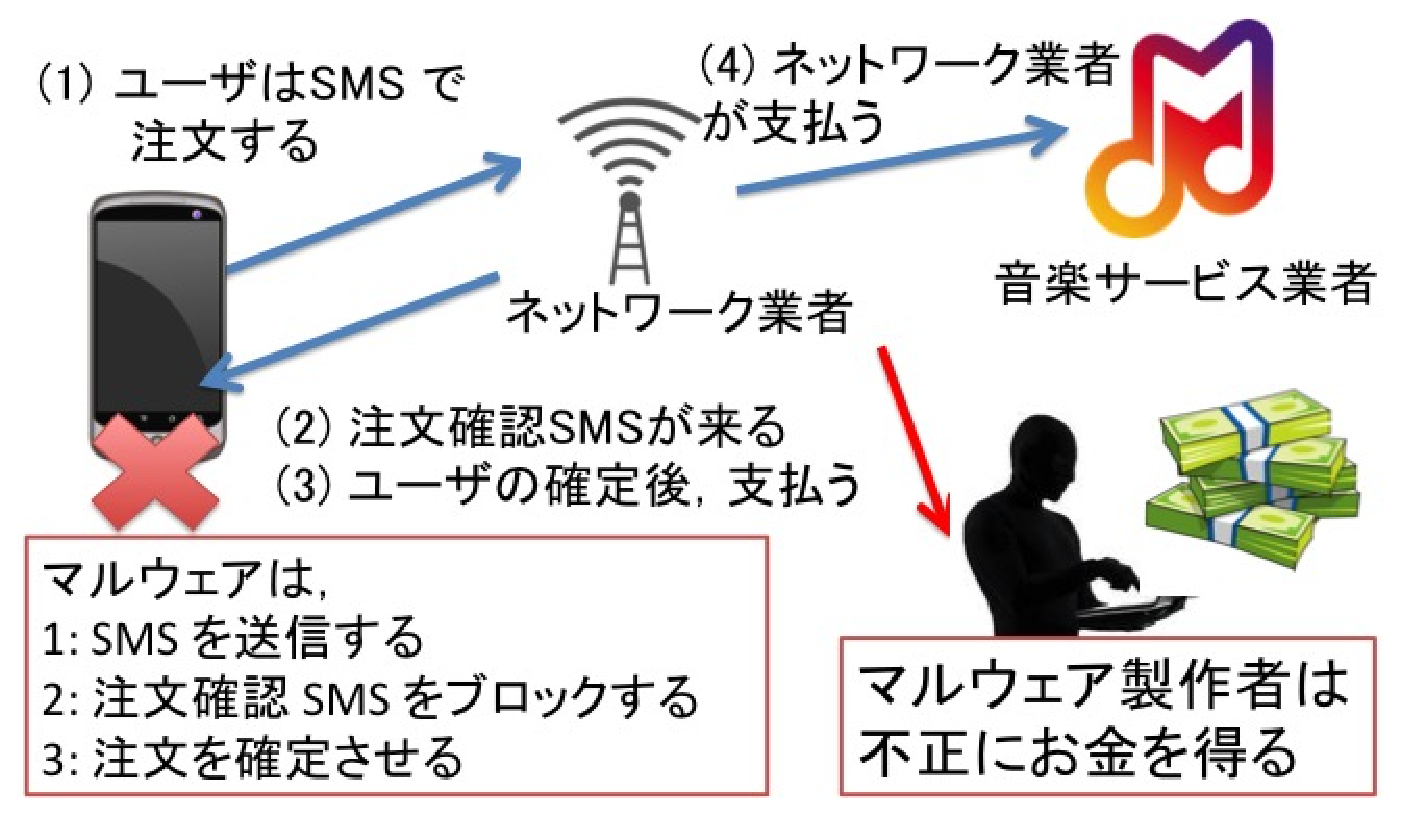
\includegraphics[ scale = 0.4]{sms3.eps}
\end{center}
\caption{SMS を使った攻撃}
\label{SmsAttack}
\end{figure}

マルウェアが先に述べたような攻撃をするための方法を 2 つ挙げる.
1 つは,外部からの遠隔操作だ\cite{remotectrl}.
マルウェアは外部サーバからの命令を受け取り,実行する.
あるマルウェアがインストールされると,外部のサーバから暗号化されたスクリプトを受け取り,そのスクリプトを復号化し,実行するという例もある.
この手法を使うと,マルウェアを検知するソフトウェアを回避することができる.
なぜなら,公式アプリケーションストア (Google Play)  にアップロードされた時点では不正な動きをするコードをマルウェア自身は何も持っていないために,このソフトウェアに検知されないからだ.
外部から得たスクリプトは DexClassLoader というクラスローダによりアプリケーションに読み込むことができる.
もう一つは,Android OS の脆弱性をつくことで,特権レベルを上げることである.
不正にマルウェア自身の特権レベルを上げるマルウェアの中には root 権限を奪うものもある.
マルウェアに root 権限を奪われてしまうと,ユーザが抵抗できる余地は少ないため,悪用されると非常に危険である.
マルウェアの 1 つである,AndroidDefender\cite{sopho}は,表向きにはウイルス対策アプリケーションとなっている.
AndroidDefender が起動すると,それは感染した端末から電話をかけられなくしたり,さまざまなアプリケーションへのアクセスを制限させる.
その後,AndroidDefender は端末を修復するためにユーザに大金を要求する.
 
実際のマルウェアの例として,GoldDream を紹介する.
GoldDream は端末情報を流出させるために,電話の発着信などのイベントを監視し,外部へと送信する.
そこで,GoldDream の挙動について説明する.
GoldDream はSMS の受信,電話の発着信があると,バックグラウンドでユーザに気づかれることなく起動される.
GoldDream はレシーバを登録することで,これらの着信が来た時に Android OS が出す通知を受け取れるようにしている.SMS を受信した際は,受信したメッセージの送り元のアドレス,内容,タイムスタンプを収集する.
電話の発着信の場合も同様に,電話番号やタイムスタンプといった情報が GoldDream によって集められる.
このような情報を利用することで,マルウェアは他の端末へ攻撃範囲を拡大することができる.
例えば,他の端末の情報を得ることができれば,感染した端末から他端末へマルウェアのダウンロードリンクを載せたメッセージなどを送ることができる.
これらの情報は一度ローカルファイルに保存された後,外部のサーバへ送信される.
GoldDream は外部サーバからコマンドを受け取り,実行する.
サーバから受け取るコマンドは,次の 4 つである.
1) SMS をバックグラウンドで送信する,2) 電話を発信する,3) アプリケーションをインストール,アンインストールする,4) ファイルをサーバへアップロードする. 
ファイルをアップロードするコマンドは端末の情報を送信するために用いられる.



\subsection{Android アプリケーションの構成}
\label{sec:andrapp}
1 つの Android アプリケーションは 1 つの APK ファイル (.apk) となってまとめられている.
Androidのアプリケーションを実行するためには,異なる種類の複数のファイルが必要である.
例えば,AndroidManifest.xml, 画像ファイル,レイアウトファイル(png, jpg, xml, etc),classes.dex, アプリケーションの証明書である.
これらを1 つのファイルに ZIP 形式でまとめたものが APK ファイルである.
そのため,zip ファイルと同様に解凍,圧縮,中身の入れ替えができる.
よって,unzip コマンド で APK ファイルを解凍することができる.
APK ファイルを解凍すると,AndroidManifest.xml, classes.dex, res ディレクトリ,META-INF ディレクトリが展開される.
res ディレクトリには,アプリケーションのアイコン画像,アプリケーション実行時に画面上に表示する画像ファイルが入っている.
META-INF ディレクトリにはアプリケーションの証明書のファイルがある.
ただし,unzip コマンドで解凍した場合,AndroidManifest.xml はバイナリのままであるため,このファイルの中身を見たい場合は,apktool\cite{apktool}というツールを使う必要がある.
これらのファイルを一つの APK ファイルにまとめるのは,他のアプリケーションも同じファイル名を用いているためだ.
どのアプリケーションも必ず AndroidManifest.xml と classes.dex の 2 つのファイルを持っている.
そのため,これらのファイルはアプリケーションごとにまとめて端末上にインストールされる必要性がある.
そうすることで,Android OS はアプリケーションを管理することができる.

AndroidManifest.xml とはアプリケーションの基本的な情報が書かれている XML 形式のファイルである.
あるゲームアプリケーションの AndroidManifst.xml の例を図\ref{manif}に示す.
アプリケーションのパッケージ名,アプリケーションが使用する権限,アプリケーションが起動した時に最初に実行されるクラスなどが記されている.
パッケージ名は OS がアプリケーションを識別する名前である.
図\ref{manif}の 2 行目に.このアプリケーションのパッケージ名 (com.gamelio.DrawSlasher) が書いてある.
パッケージ名は待ち受け画面でアイコンの下に表示される名前とは異なる.
例えば,Facebook,Instagram の Android アプリケーションの場合はそれぞれ,com.facebook.katana,com.instagram.android となっている.
一般的にアプリケーションを使用している分には,ユーザはパッケージ名について気にする必要がないので,Android 端末を使用していてアプリケーションのパッケージ名を目にすることはまずない.
ただし,Android Debug Bridge (adb) を用いてターミナルからアプリケーションを手動でアンインストールする場合は,パッケージ名を特定する必要がある.
OS monitor という Android のシステム状況を確認できるアプリケーションを使うと,AndroidManifest.xml を見なくても,実行中のアプリケーションのパッケージ名を端末上で見ることができる.

Androidのアプリケーションは OS から権限を得ないと実行できないことがいくつもある.
たとえば電話の着発信,SMS の送受信, インターネットへの接続などである.
AndroidManifest.xml にこれらの権限を記すことにより,アプリケーションはその権限を得る.
これらの機能をアプリケーションで実行するためには,必ず AndroidManifest.xml に宣言しないといけない.
図\ref{manif}の中では,24 行目から38 行目にかけてこのアプリケーションの権限が書かれている.
さらに,マルウェアの AndroidManifest.xml を得ることができれば,どのようなことをしようとしているのかがわかる.
表向きは電話帳のデータとは関係の無いアプリケーションであるのに,AndroidManifest.xml で電話帳へのアクセスの権限を要求していたら,何らかの不正な動きをするアプリケーションである可能性であることが高い.
図\ref{manif}の 34 行目には,電話をかけるための権限である,CALL\_PHONE が宣言されている.
このアプリケーションがマルウェアではない,安全なゲームアプリケーションであるとすれば,電話を発信する必要はない.
つまり,このアプリケーションは電話をかけることで何らかの不正な動きをする可能性が高い.
 
 AndroidManifest.xml ではアプリケーションが起動したときに最初に実行する activity を指定する必要がある.
図\ref{manif}の 7 行目から,最初に実行される activity は com.Claw.Android.ClawActivity ということがわかる.
この指定が無いと Android OS はどこから実行すればよいかわからない.
activity とは 1 画面を表すクラスであり,Android アプリケーション内で画面が変わるということは,他の activity に変わる(遷移する)ということである.
画面内でボタンなどを表示させたいときは,android.Activity クラスをオーバーライドして,実装する.
このように,AndroidManifest.xml はアプリケーションの大まかな概要を示している.

アプリケーションの画像ファイルが入っている res (resource) ディレクトリ内には様々なファイルがあり,その種類に応じて配置されるディレクトリが決まっている\cite{resource}.
図\ref{res}は,あるアプリケーションの res ディレクトリの構成を示したものである.
layout  ディレクトリでは,ユーザインターフェース (以下 UI) のレイアウトを定義する XML ファイルが入っている.
レイアウトリソースファイルはアプリケーションの activity の UI の構成を決めている.
例えば,テキストを表示する領域を表す TextView の縦幅と横幅の具体的な値が記されている.
drawable ディレクトリには画像ファイル (.png, .jpg, gif etc) と形状などを定義した XML ファイルがある.
drawable ディレクトリにある XML ファイルはボタンを押した時などの状態変化のために用いる.
図\ref{res}では,drawable ディレクトリがいくつも分かれている.
これは,異なる解像度に対応するためである.ldpi は Low-density,mdpi は Medium-density,xhdpi は Extra-high-density, xxhdpi は Extra-extra-high-density を表す.
menu ディレクトリにはアプリケーションのメニューの内容を定義する XML ファイルが.values  ディレクトリには文字列,数値,色などの値を定義する XML ファイルが入っている.

classes.dex は,Android アプリケーションの DEX コード実行ファイルである.
DEX コードとは,Android 上で動く VM,Dalvik VM の中間言語だ.
Android アプリケーションの APK ファイル内には,必ず classes.dex は 1 つしか存在しないことになっている.
二つ以上の .dex ファイル(例えば,classes.dex と classes1.dex)を APK ファイル内に入れることはできるが,実行するときは classes.dex のみが実行される.
アプリケーションのソースコードの全てのクラスファイルの中身が 1 つの DEX コードに変換される.
Java Virtual Machine (JVM) も中間言語である,Java バイトコードを用いている.
Javaでは,コンパイル時にクラス毎に Java バイトコードのファイル,クラスファイルが生成される.
しかし,Dalvik VM では,アプリケーションごとに DEX コードのファイル (classes.dex) が生成される.
アプリケーションの Java ファイル (.java) はコンパイルされて Java クラスファイル (.class) に変換される.
その後,そのクラスファイルが 1 つの DEX コードファイルにまとめられる.
つまり,Android 端末内でアプリケーションが実行されるときには Java で実装されたソースコードのクラスとは関係なく,1 つの実行ファイル,classes.dex が Dalvik VM 上で実行される.
また,dex2jar\cite{d2jar}というツールにより,classes.dex を JAR 形式に変換することができる.
JAR ファイルは Java バイトコードが圧縮されたファイルであるから,これを解凍することで,Android アプリケーションのクラスファイルを手に入れることができる.
また,Android SDK が提供する dx というコマンドラインツールを用いることで,jar ファイルから DEX コードファイルを作成することもできる.
本提案ではこれらの方法を用いてマルウェアのクラスファイルを入手し,そこから classes.dex を作成した.


\begin{figure}[t]
\begin{center}
\graphicspath{{./epsfiles/}}
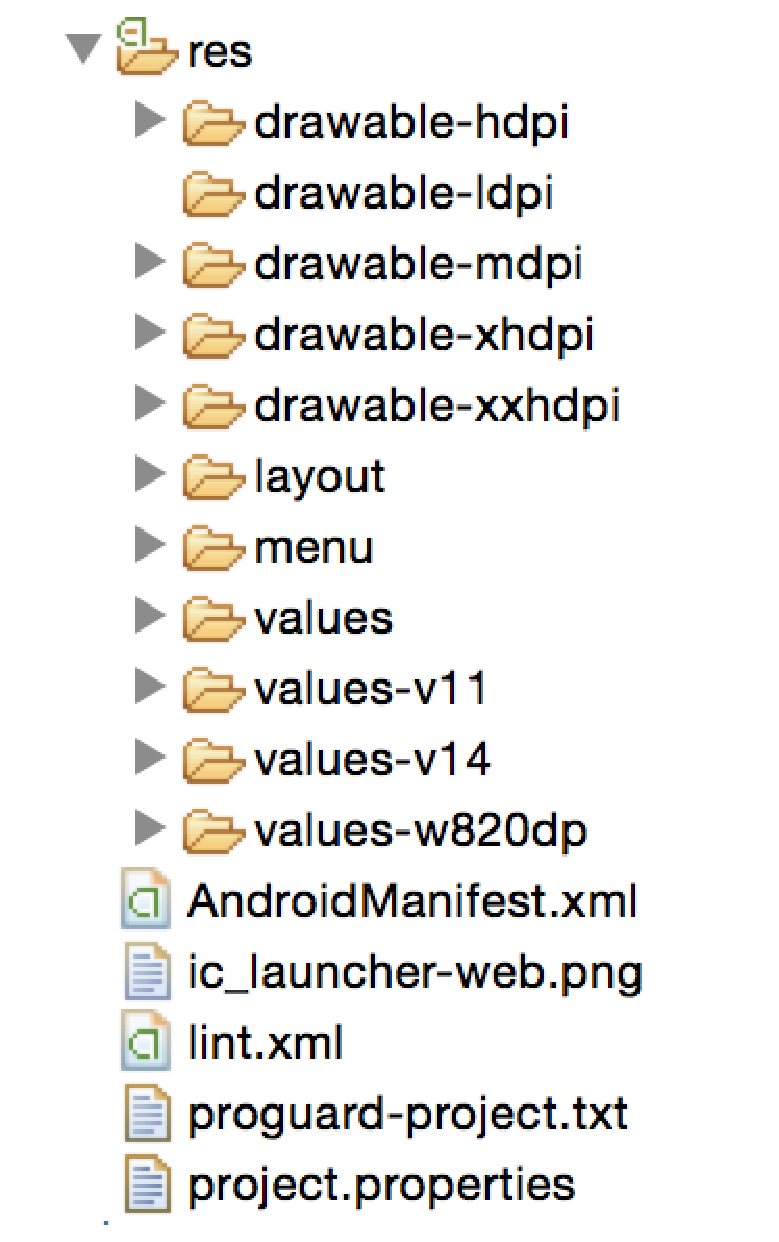
\includegraphics[ scale = 0.2]{resource.eps}
\end{center}
\caption{ res ディレクトリの構成}
\label{res}
\end{figure}

\begin{figure}[t]
\begin{center}
\graphicspath{{./epsfiles/}}
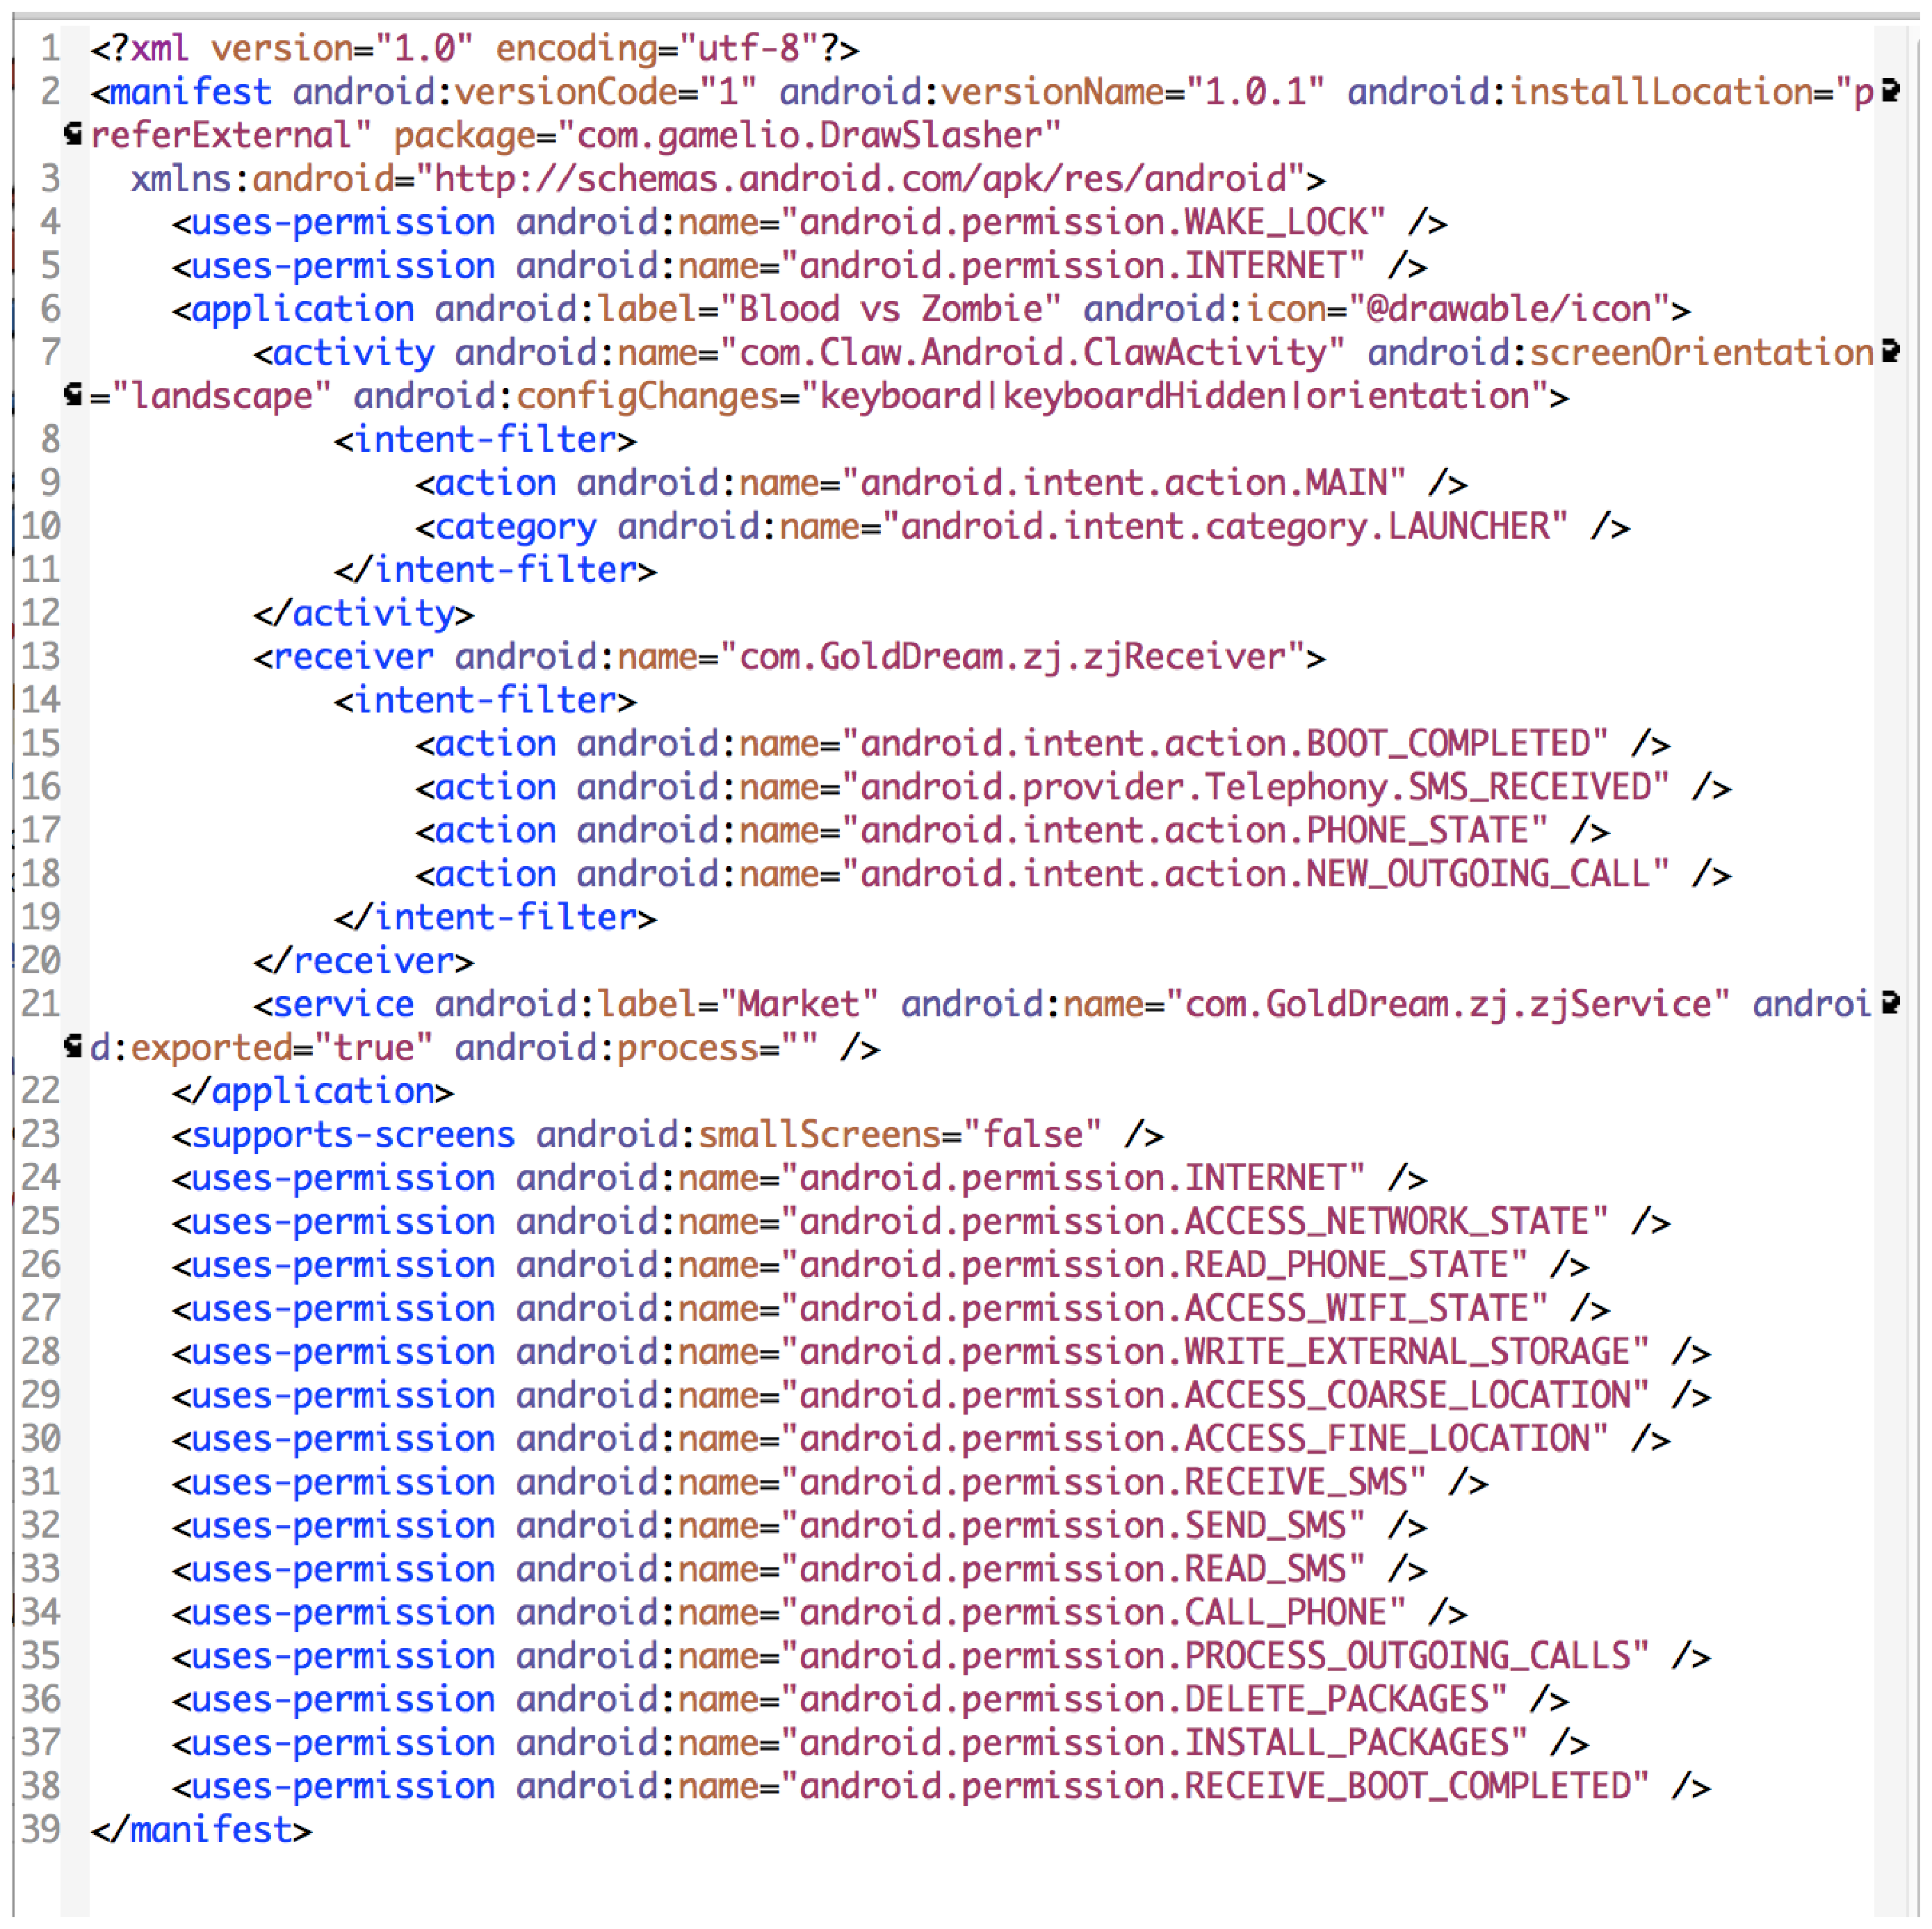
\includegraphics[scale=0.25]{manifest2.eps}
\end{center}
\caption{AndroidManifest.xml の例}
\label{manif}
\end{figure}


\clearpage

\section{関連研究}
\ref{tools} では \ref{sec:intro} 章で述べた,androguard, droidbox についてより詳しく説明する.\ref{researches} で,Android マルウェアを解析,調査した研究を 3 つ紹介する.
\subsection{Android マルウェアを解析するためのツール}
\label{tools}
androgurard \cite{aguard} は Android マルウェアを解析し,クラス同士の関係を表すグラフを作る.このAndroid アプリのクラスの視覚化ツールは Androgexf である.androguard  は Androgexf だけではなく,他にもたくさんのツールを提供しており,その数は全部で 14 にもなる.その中の 1 つの Androaxml は\ref{sec:andrapp} で説明した,AndroidManifest.xml などのバイナリーの XML を人間が読めるように変換するツールである.Androgexf  に APK ファイルを入力すると,GEXF 形式のファイル (.gexf) として解析結果のグラフを出力する.GEXF ファイルは Gephi というフリーソフトで見ることができる.このグラフはメソッドコールグラフであり,それぞれのノードには,メソッドのタイプ (activity, service, receiver etc) , クラス名,どの権限が使用されているか,その権限のレベル (それぞれの権限には,normal, signature, dangerous などのレベルがある) が記されている.図\ref{androguardgraph} のように,このグラフではどの部分が危険であるかを色を変えて示してあり,どのメソッドが不正な動きをしているかがグラフを見れば簡単にわかる.図\ref{androguardgraph} では,"MONEY\_RISK", "SMS\_RISK" というタグが付けられている.これは,矢印が指されているメソッドのノード,sendSms がバックグラウンドで SMS を送るという危険があることを示している. また,動的にコードをロードしているメソッドも検知することができる.

droidbox \cite{dbox} は Androidのエミュレータ上でマルウェアを実行することで動的に解析する.droidbox  は,端末のネットワークデータのやりとり,ファイルの読み込み・書き込みの命令,ネットワーク,ファイル,または SMS を通じた情報の流出,送信された SMS と電話,開始されたサービス,といった多くの情報を解析する.さらに,解析後は,マルウェアの振る舞いを表す 2 つのグラフも生成する.図\ref{dboxgraph1} , 図\ref{dboxgraph2} はこの 2 つのグラフである.図\ref{dboxgraph1} の縦軸はアプリの活動の種類を表し,横軸は時間である.図\ref{dboxgraph1} の 横軸  30 から 40 にかけて,"net open", "leak" という activity が頻繁に発生している.これはこの間に情報が流出したことを意味する.図\ref{dboxgraph2} は解析した複数のマルウェアの類似性を比較するために用いられる.それぞれの色 (CALL, FILE WRITE, NETLEAK, etc) の領域の割合を比べることで,異なるパッケージのマルウェアがどれほど似た挙動をしているかがわかる.

\begin{figure}[t]
\begin{center}
\graphicspath{{./epsfiles/}}
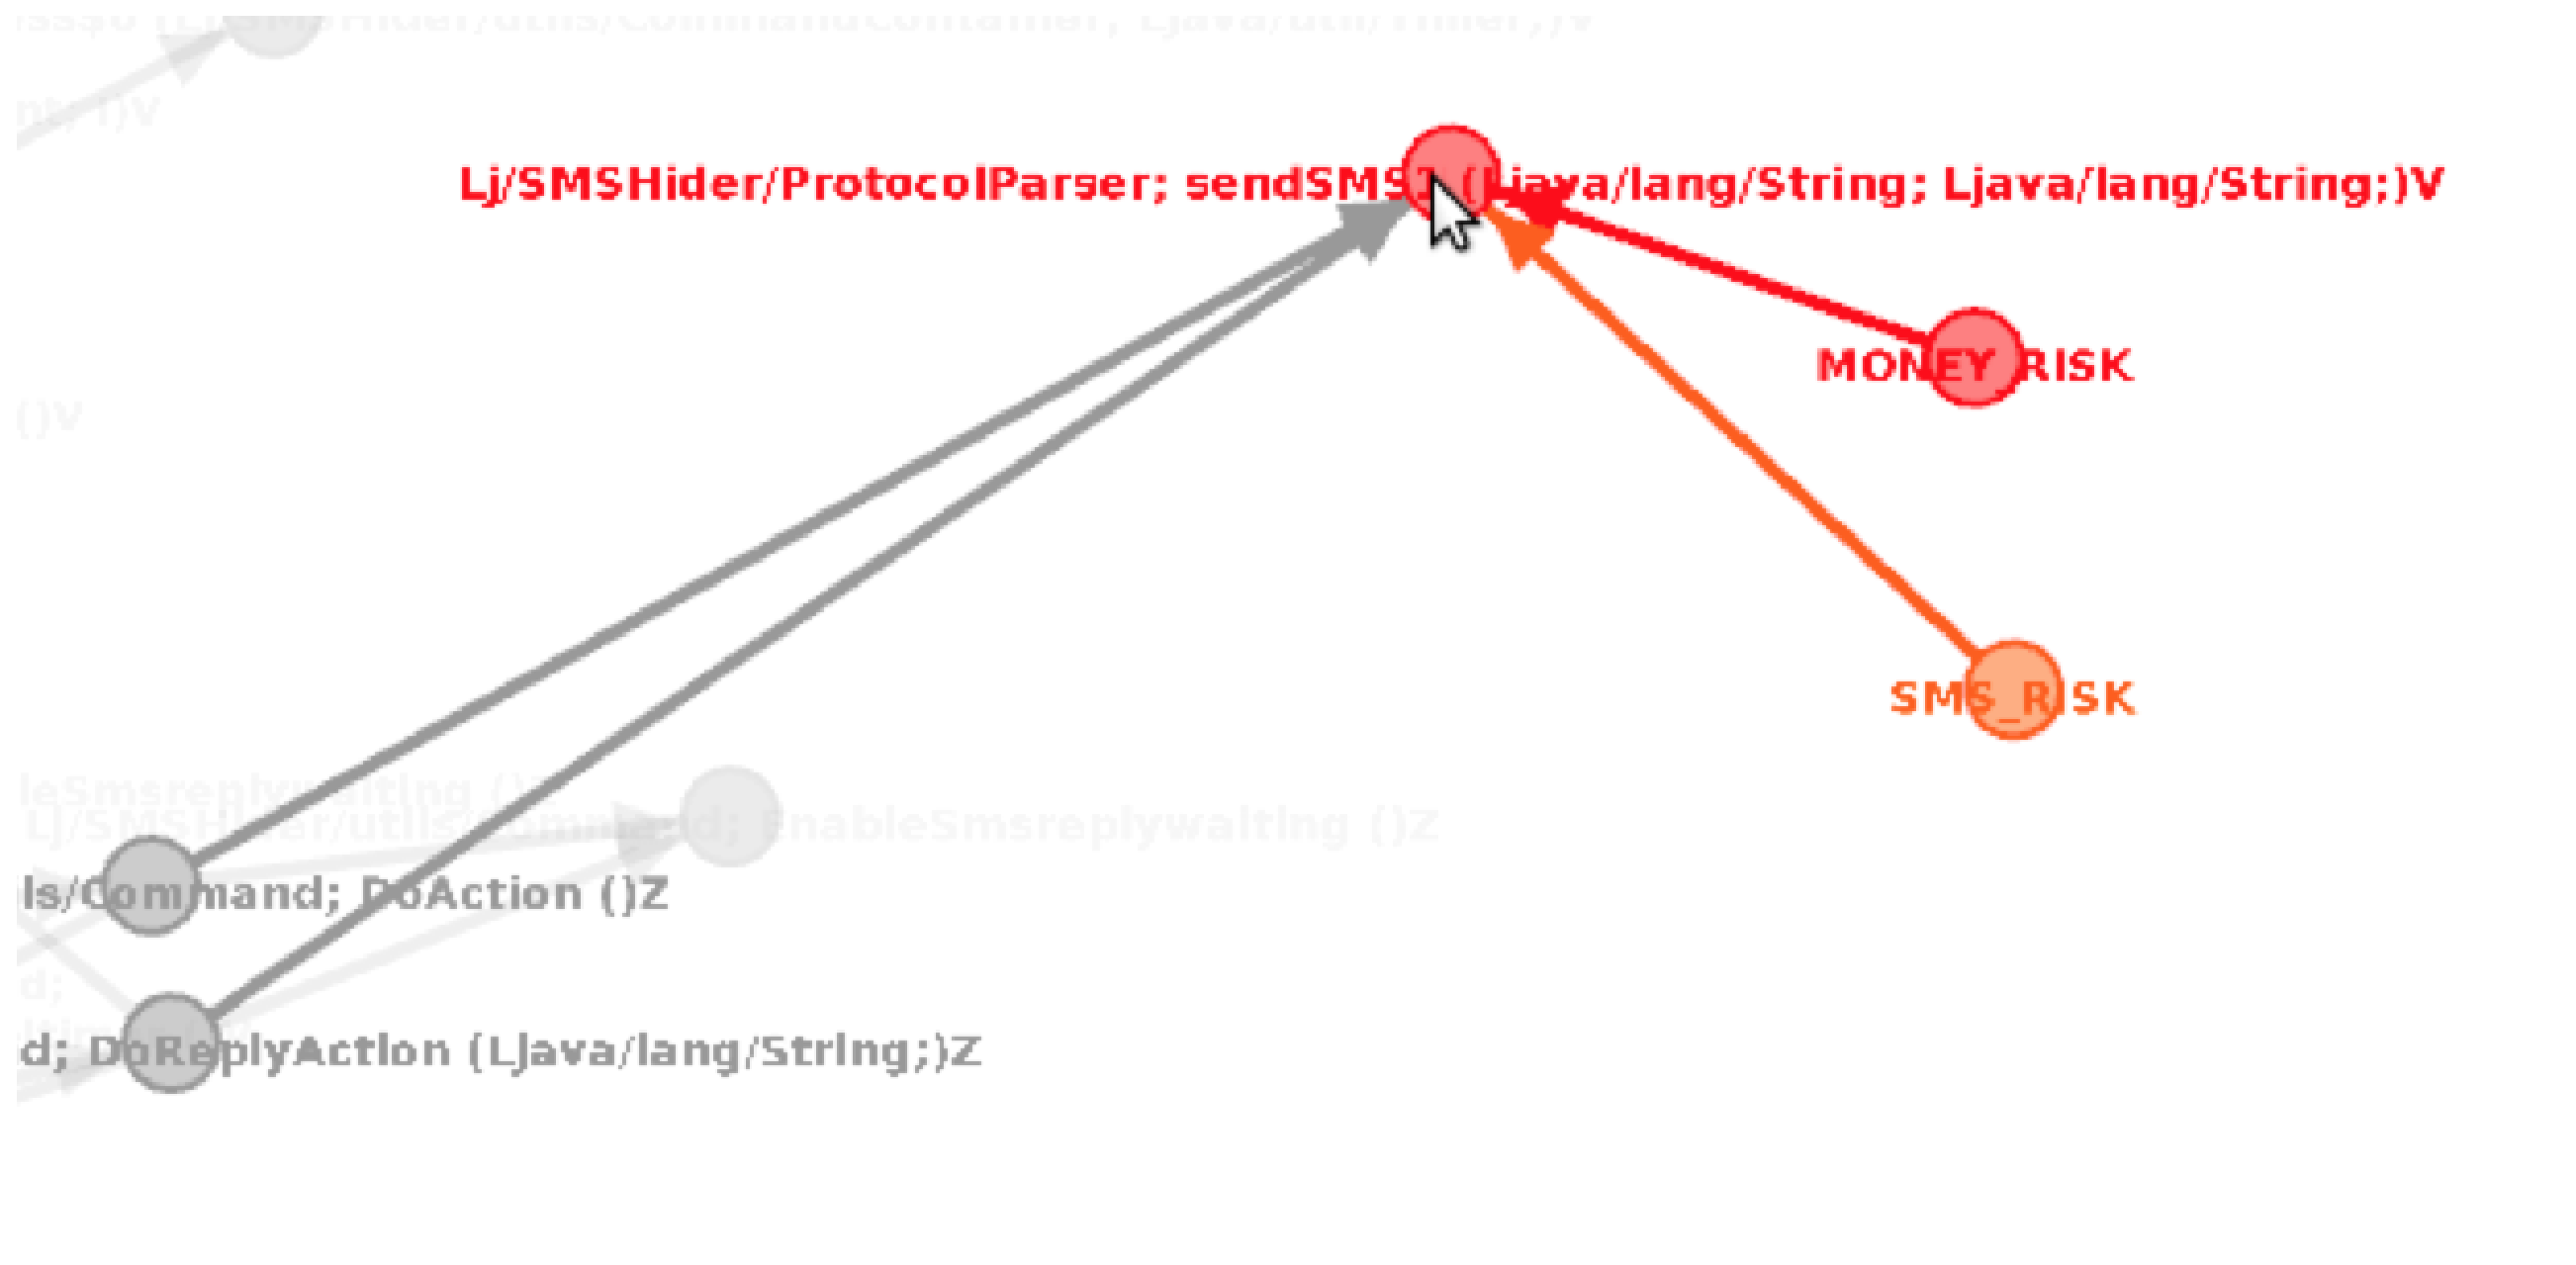
\includegraphics[ scale = 0.3]{androguard.eps}
\end{center}
\caption{androguard が生成するグラフの一部}
\label{androguardgraph}
\end{figure}

\begin{figure}[t]
\begin{center}
\graphicspath{{./epsfiles/}}
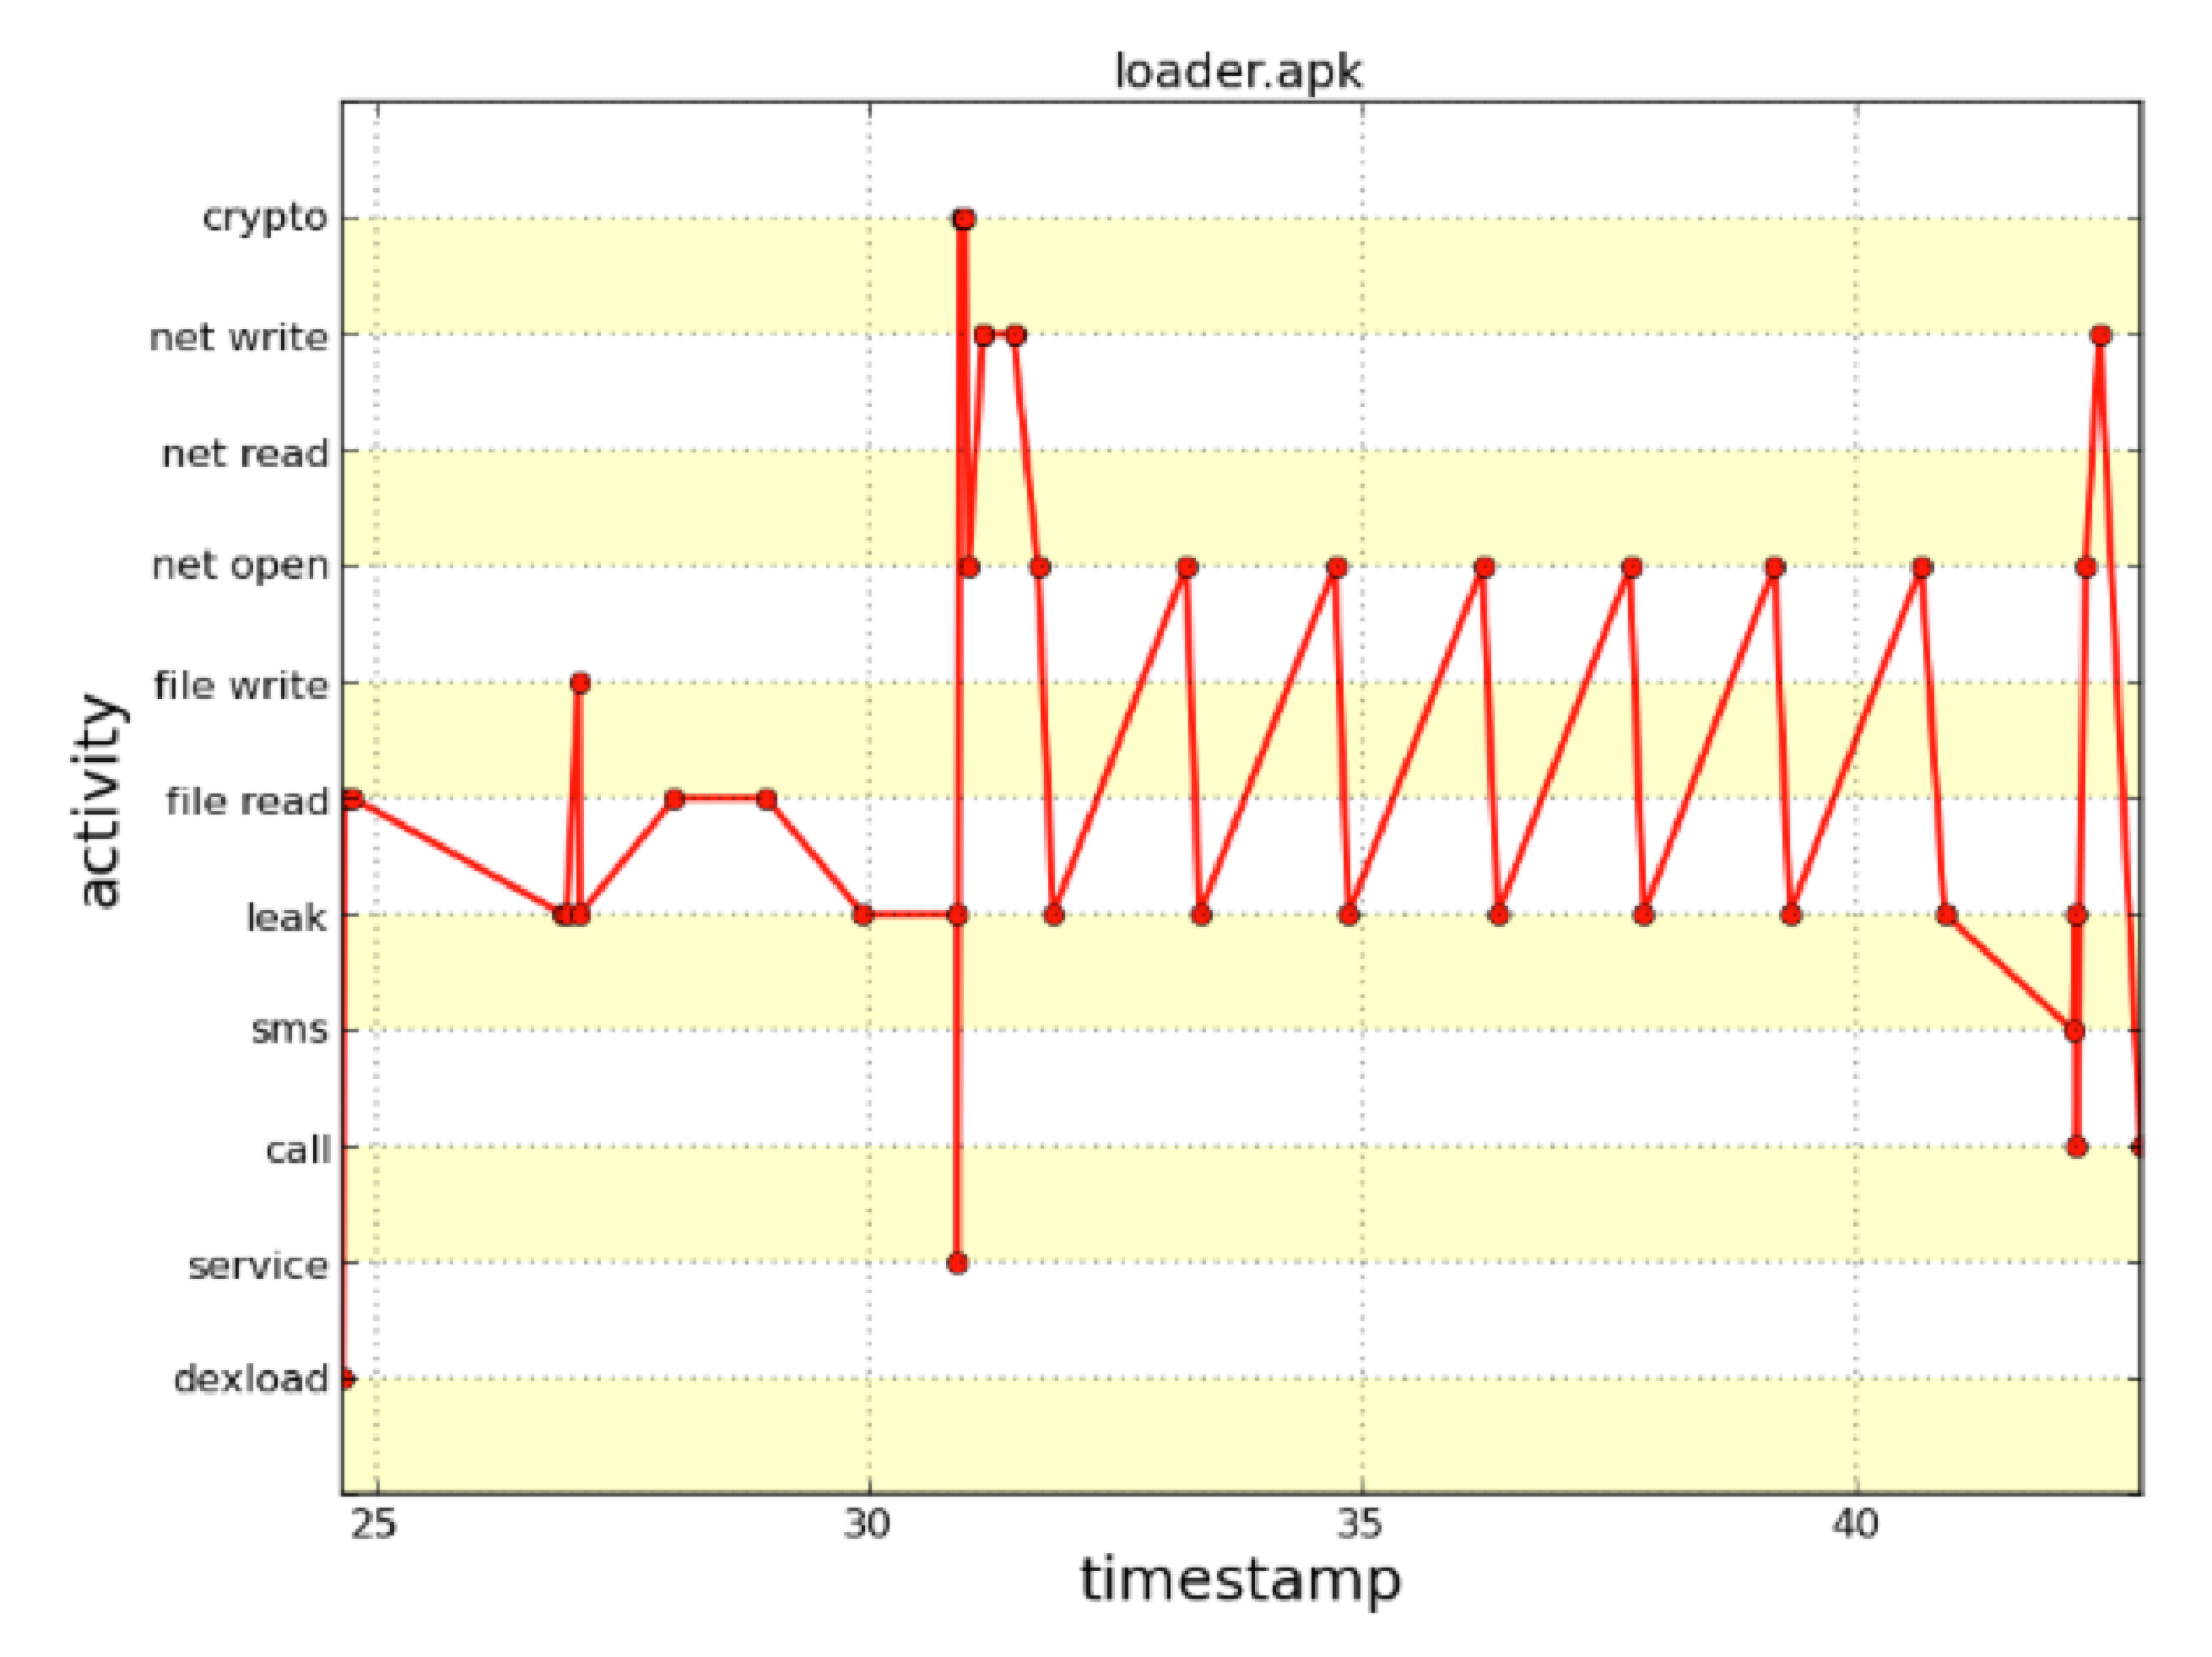
\includegraphics[ scale = 0.2]{droidbox1.eps}
\end{center}
\caption{droidbox の activity の時系列グラフ}
\label{dboxgraph1}
\end{figure}

\begin{figure}[t]
\begin{center}
\graphicspath{{./epsfiles/}}
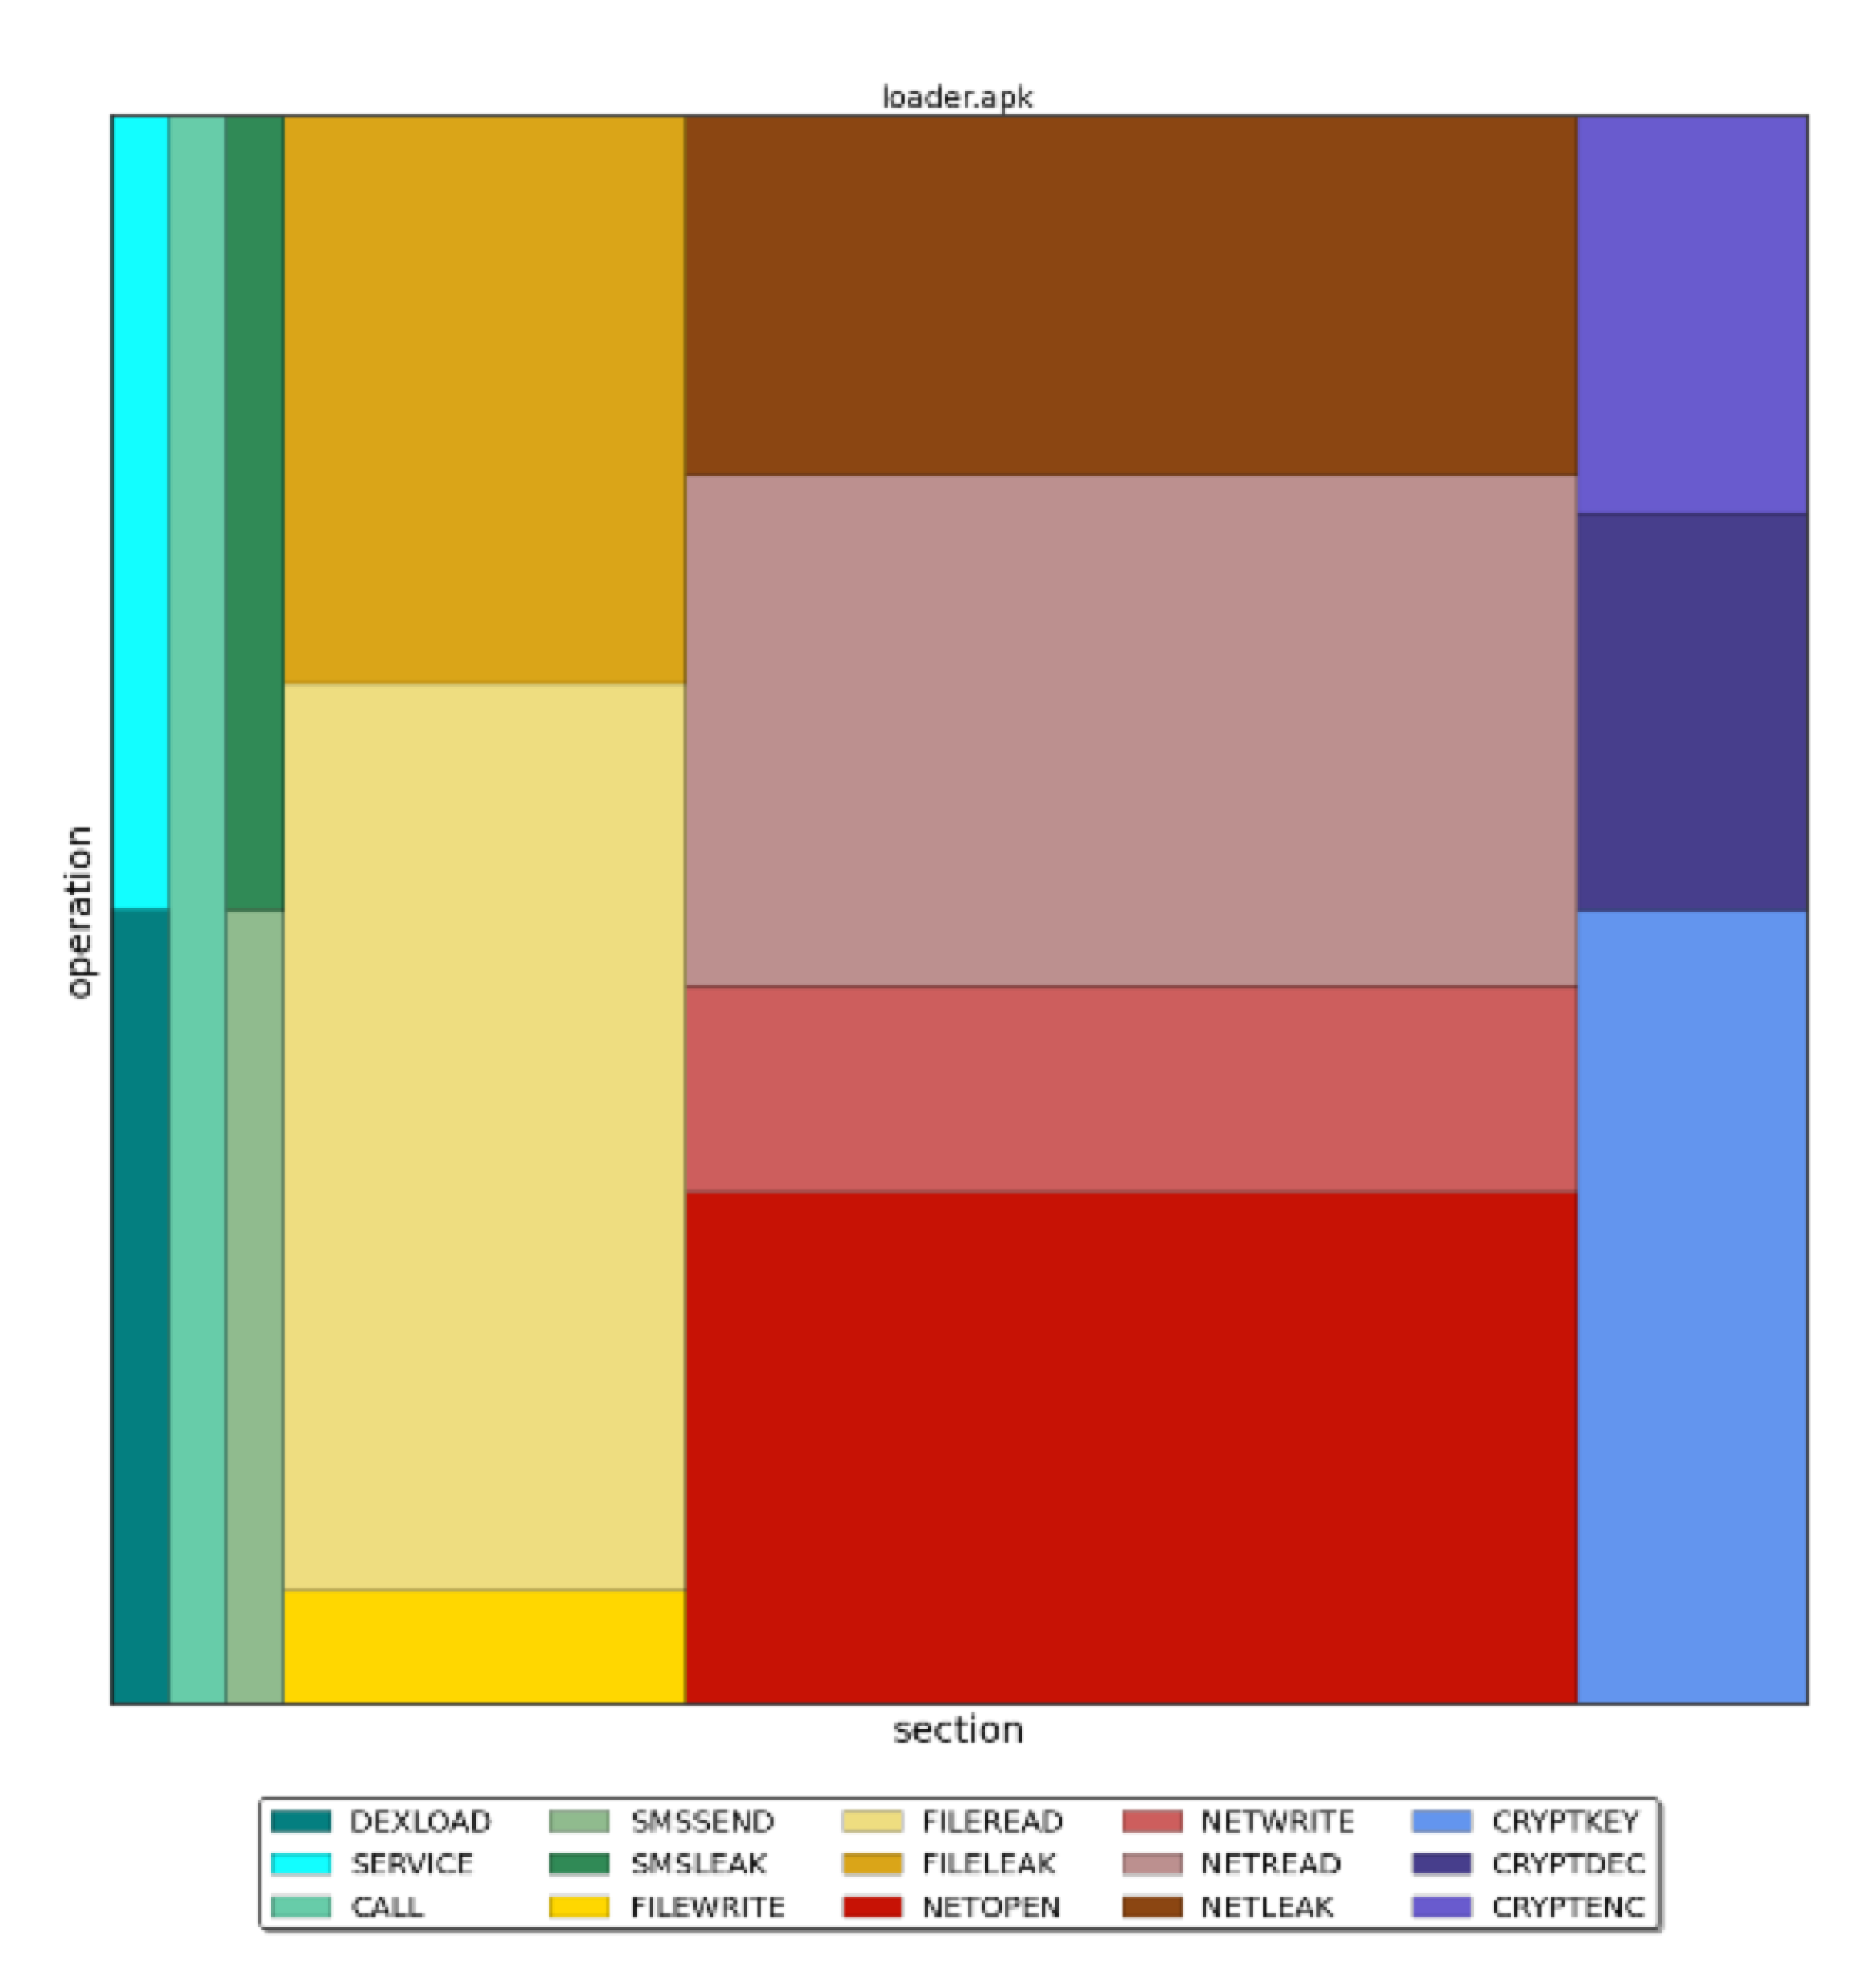
\includegraphics[ scale = 0.2]{droidbox2.eps}
\end{center}
\caption{droidbox の operation - section グラフ}
\label{dboxgraph2}
\end{figure}

\if0
\begin{figure}[t]
	\begin{minipage}{0.5\hsize}
	\begin{center}
		\graphicspath{{./epsfiles/}}
		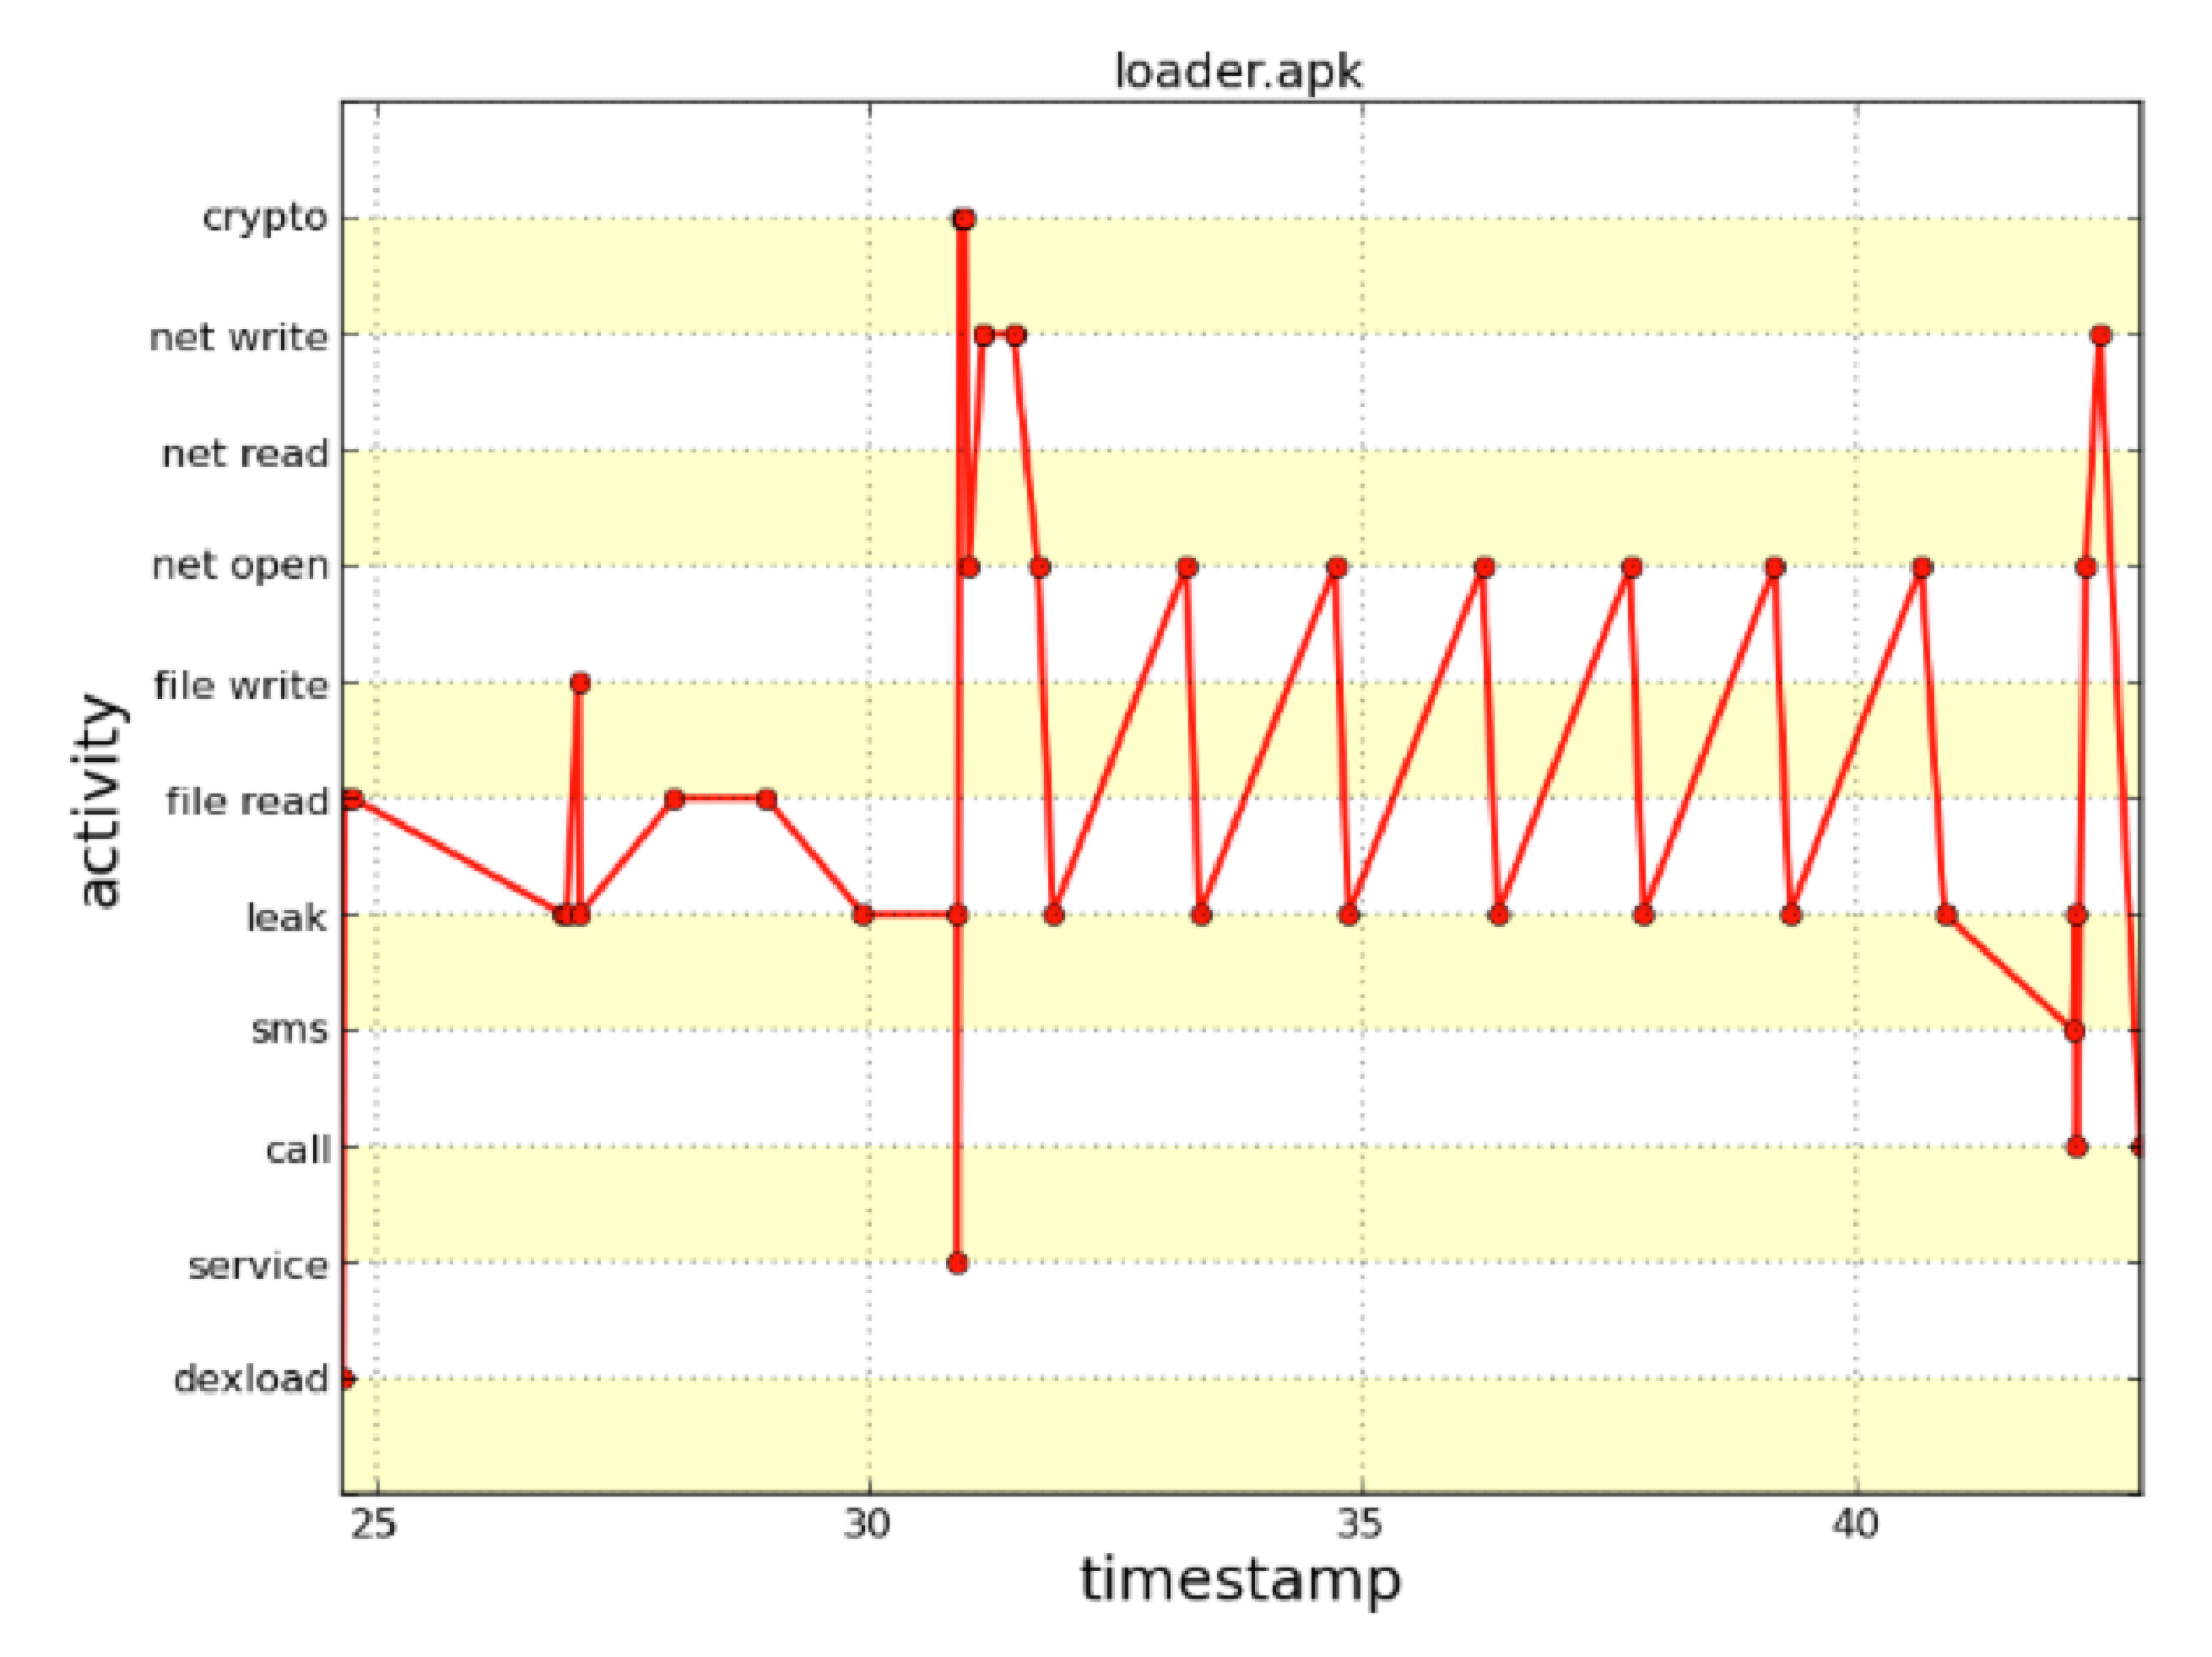
\includegraphics[scale=0.2]{droidbox1.eps}
	\end{center}
	\end{minipage}
	\begin{minipage}{0.5\hsize}
	\begin{center}
		\graphicspath{{./epsfiles/}}	
		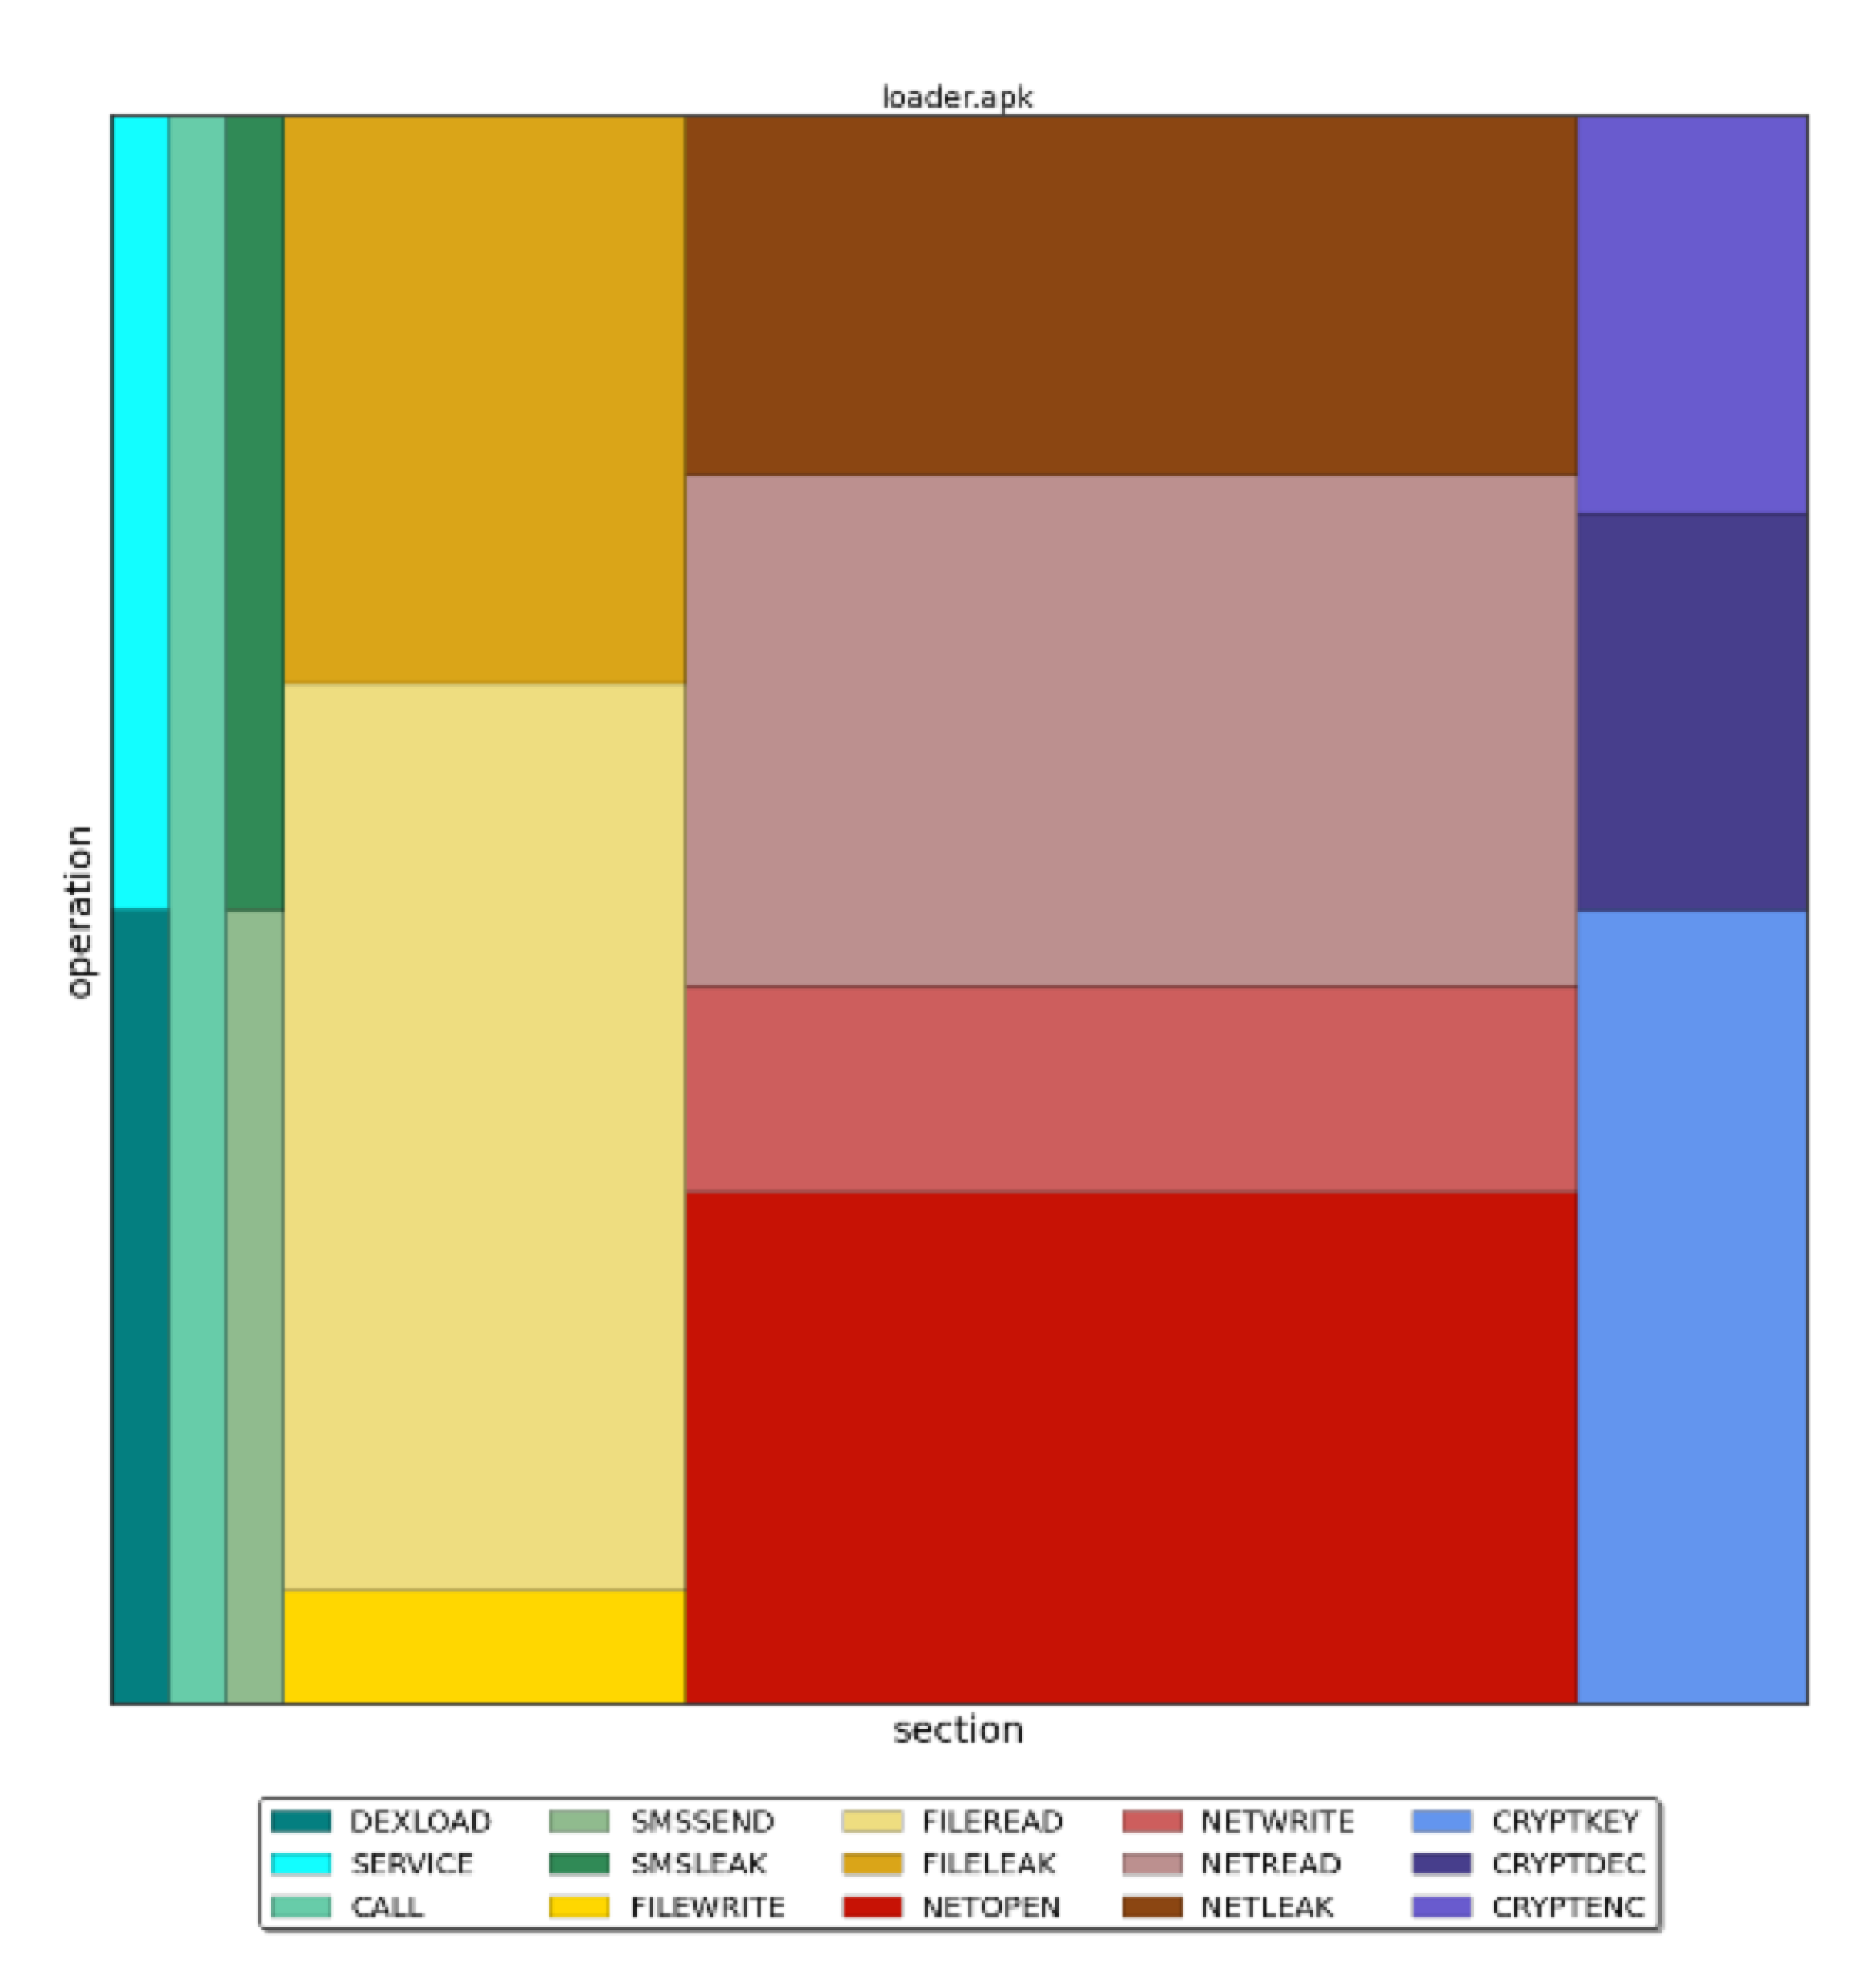
\includegraphics[scale=0.2]{droidbox2.eps}
	\end{center}
	\end{minipage}
\caption{droidbox  が生成するグラフ}
\label{droidboxgraph}
\end{figure}
\fi

\subsection{Android マルウェアを解析,調査した研究}
\label{researches}
Y.Zhou, X.Jiang は,2010 年の 8 月から 2011 年の10 月にかけて,公式サイト,非公式サイトから収集した 1,260 個,49 種類のAndroid マルウェアを用いて時系列調査と分類調査を行っている \cite{dissect} .時系列調査では,この研究で収集しているマルウェアの数 (dataset) をグラフで示している.図\ref{dataset} は その dataset の推移を表すグラフである.DroidKungFu が登場した 2011 年 6 月,AnserverBot が登場した 2011 年 10 月にこの dataset の数が急激に増えた.つまり,この 2 つのマルウェアが大きな影響を及ぼしていることがわかる.分類調査では,マルウェアのインストールの方法,起動トリガー,挙動,マルウェアが要求する権限を調査している.49 種類中,25 種類のマルウェアが Repackage によりインストールされていた.マルウェアの起動トリガーとして最も多かったのは,OS の起動時で,29 種類だった.マルウェアの挙動は,Financial charge が最も多く,その中でも,SMS を使っているものが多かった.また,多くのマルウェアが SMS, Wi-Fi に関する権限を要求していた.また,先に出てきた,2 つのマルウェアがどのような挙動をするかを示している.DroidKungFu は6 種類のヴァージョンが見つかっており,外部サーバのアドレスの格納方法が暗号化によって複雑化している.そのため,全く意味の無い文字列でも暗号化されている可能性があるのでこれらを復号して確認する必要が出てくる.よって,解析により手間がかかり,さらに難しくなってしまう.AnserverBot は解析回避と遠隔操作の2 つの特徴を持つ.AnserverBot は解析回避のために 2 つの方法をとっている.一つは自身が解析されているかどうかを検知する方法で,もう一つはメソッド名やクラス名を意図的に変えることで解析を行いにくくする方法である.

さらに,彼らは既存の 4つのセキュリティソフトがこの  dataset を検知するかどうかの調査も行った.その結果,最高は Lookout の 79.6 \% , 最低は Norton の 20.2 \% で,どのソフトウェアも検知できないマルウェアも存在した.この結果より,この 4 つのセキュリティソフトはまだ不十分であることがわかる.これらの調査結果からこの研究の結論として,マルウェアのインストール方法の中でも,最も頻繁に行われている Repackage を検知することとアプリの外部のコードの動的ローディングを防ぐ技術が必要であると彼らは主張している.この研究は Android マルウェアを調査,分類し,さらに 2 つのマルウェアについて詳しく挙動を示している.この研究では,解析手段(静的か動的か)までは言及していない.本研究では調査,分類を行うために必要となるさまざまな種類のマルウェアの挙動を正確に解析する手法を提案する.


S.Poeplau らは,マルウェアの動的に外部コードの動的ローディングに焦点をおいて解析を行っている \cite{dynamicloading} . \ref{sec:malware} で述べたように,外部コードのローディングをすることで公式ストアの検知システムをくぐり抜けることができる.また,外部コードのローディングは必ずしも不正なものではなく,マルウェア以外のアプリでも使われている.しかし,Android OS はロードされたコードをチェックしないので攻撃者はロードするものを置き換えることができる.そのためこれは Android アプリの脆弱性といえる.そこで,この研究で彼らは外部コードの動的ローディングを検知するツールを提案している.このツールは APK ファイルから取り出した DEX コードを静的に解析する.100 万回以上インストールされた,1,632 個のアプリをランダムに選び,このツールを用いて検査した.その結果,その中の 9.25 \% から外部コードのローディングの脆弱性が検知された.さらに,Google Play  での人気 50 位以内の無料アプリを同じツールで検査すると,16 \% ものアプリがその脆弱性を示した.また,彼らはこの攻撃手法に対する防御策も提案している.Dalvik VM が外部からダウンロードされたコードのハッシュ値を計算し,それが Whitelist に載っていなければ,それを実行できないようにアプリケーションに制限をかける.そうすることで,これを利用した攻撃を防ぐことができる.
外部コードの動的ローディングの応用例として,文字列としてクラス名,メソッド名を受け取り,Java の reflection を通して実行することが考えられる.reflection  とは,プログラムの実行時においてプログラム自身の構造を読み取ったり書き換えたりする技術のことである.彼らの研究では外部コードの動的ローディングの攻撃を防ぐツールを提案したが,reflection を使うと,このツールでは検知することができない.
この研究では静的解析を行っているために,外部コードのローディングは検知するが,外部コードの挙動が悪意あるものかどうかは解析しない.上記でも述べたように,外部コードのローディングは必ずしも悪意あるものとは限らない.それに対して本研究では,動的解析を行っているためにこのような外部コードの動的ローディングによる悪意ある挙動を解析することができる.


L.Yan, H.Yin はマルウェアの動的解析環境 (DroidScope) を提案している \cite{droidscope} .彼らは Android SDK が提供するエミュレータをベースに自分たちで手を加えて,そのエミュレータの中でマルウェアを動かしている.彼らは Android システム全体の再構築を行っている.つまり,DroidScope はハードウェア,Linux OS (Android は Linux をベースにして動作している),Dalvik VM の 3 種類の API を提供する.DroidScope が提供する API を用いることで,Android API, Dalvik VM, Linux , さらには機械語の命令までをトレースするツールを提案している.{\it API tracer, native tracer, Dalvik instruction tracer} の 3 つである.また,これらの API に動的な taint analysis を実行することで,情報漏えいを解析するツール ({\it Taint tracker}) も提案している.彼らはこの 4 つのツールのパフォーマンス測定も行っている.元のエミュレータで実行時間を基準に,4 つのツールの実行時間を調べた.その結果,オーバーヘッドは小さいと言える結果であった.しかし,taint traker は他の 3 つのツールとくらべて大きなオーバーヘッドを示した.彼らはこれらのツールを用いて先に述べた,DroidKungFu を解析した.この解析によって,このマルウェアのルート権限を取得する方法と情報を盗み出す方法を明らかにしている.DroidKungFu だけでなく,論文中では DroidDream も解析している.DroidKungFu の場合と同様な解析を行った結果,DroidDream が端末識別番号を盗み出す方法を突き止めた.DroidScope は 1 つの実行パスのみを解析しない.彼らは実行パスを増やすために,システムコール,ネイティブ API,Dalvik メソッドなどの返り値を変えることで,異なる実行パスを実現した. symbolic execution のほうが,より良いことが考えられるが,かれらはこれを今後の課題としている.彼らの研究は実行された API,メソッドを動的に得ることで解析を行っているため,解析のためのアプローチは本研究と共通している点がある.しかし,本研究は実機で行っているのに対して,彼らの研究はエミュレータ上で行っている.もし,マルウェアがエミュレータ上で動作しているのを検知して,振る舞いを変える可能性もある.デスクトップ PC を標的にしたマルウェアは実際に振るまいを変えることがわかっている \cite{detection} \cite{emulation} \cite{v2e} . DroidScope のような解析ツールが普及するにつれて,エミュレータでの実行を検知するマルウェアが出てくるだろうと,彼らはこの論文中で述べている.本研究が提案している実機による解析であればマルウェアの "正常" な動作を解析することができる.

マルウェアを解析している方法としては,動的解析と静的解析がある.S.Poelau らは外部コードの動的ローディングを用いるマルウェアを静的解析により検知する手法を提案している.しかし,静的解析であるために,実際に外部からコードを受け取ってその結果実行されるマルウェアの挙動を解析することはできない.L.Yan, H.Yin が提案する DroidScope はエミュレータ上で動的にマルウェアを解析している.エミュレータで実行する場合と実機で実行する場合では,厳密に同じ環境であるとはいえない.エミュレータでの解析を検知する機能を持ったマルウェアが将来出てきた場合,DroidScope はマルウェアを解析することができなくなってしまう.そこで,本研究では実機でマルウェアを実行して解析を行う.

\begin{figure}[t]
\begin{center}
\graphicspath{{./epsfiles/}}
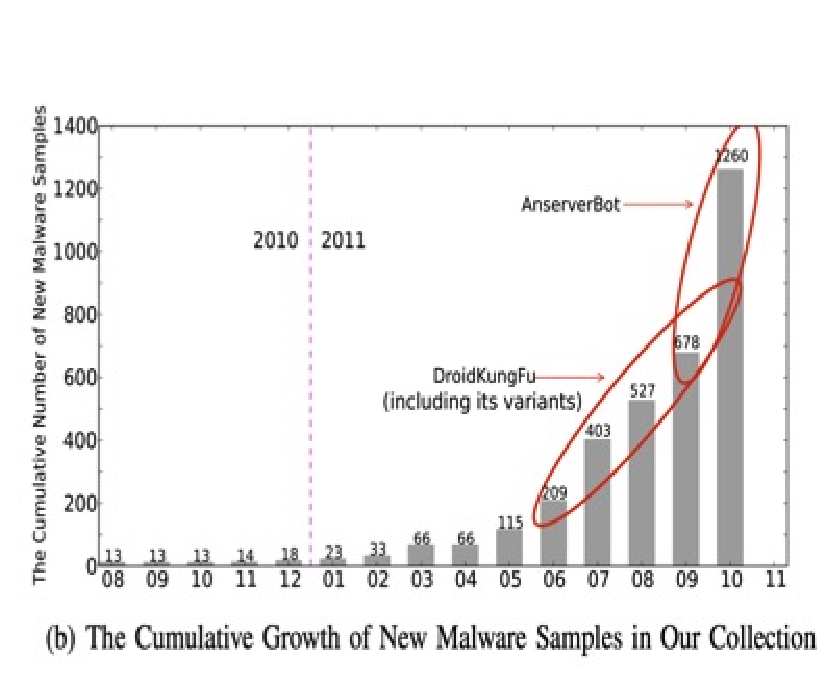
\includegraphics[ scale = 0.5]{graph.eps}
\end{center}
\caption{マルウェアの dataset の推移}
\label{dataset}
\end{figure}

\clearpage

\section{提案}
本研究では,Android を標的にしたマルウェアの動的解析を行う.マルウェアにログコードを挿入させ,そのログを動的に得ることで解析を行う.エミュレータでは再現できないために解析できないことも,本提案を適用することで,実機でマルウェアを動かすため解析できるというメリットがある.\ref{overview} では,本提案の全体の流れを説明する.\ref{analysismethod} では,本提案の解析手順を,\ref{placeinsert} では,ログコードをどこに挿入するかについて説明する.

\subsection{概要}
\label{overview}
本研究で対象とする Android アプリのマルウェアを解析するためにはメソッドの情報が必要である.解析を行っていくためには,マルウェアがどのようなコードが実行したかということを知る必要がある.Android アプリのマルウェアは Java で実装されているため,解析の手がかりとなるのはメソッドのログである.このログにはマルウェアがどんなメソッドを実行したかという情報とそれぞれのメソッドについての情報が含まれている.メソッドの情報とは具体的にいうと,メソッド名,そのクラス名,引数の型名と値である.本提案では,このログを用いてマルウェアの解析を行う.

本提案では,先に述べたログを得るためにマルウェアのメソッドにログを出力させるコードを挿入する.Android API では,デバッグ用等のために,ターミナルにログを出力する API を提供している.その API とは android.util.Log である.以下に示す例のようなコードをメソッドの中に挿入する.Log.d の ".d" は "DEBUG" を表しており,Android のログの重要度を示している.ログコードを挿入してマルウェアを実行させると,マルウェアがそのメソッドを実行したときにそのログコードは必ず実行される.よってメソッドについてのログを出力させることができる. \ref{analysismethod} では,どのようにコードを挿入するかの手順について説明する.

\begin{itembox}[l]{android.util.Log の例}
	Log.d("Tag", "Log Message");
\end{itembox}

本提案では,まずマルウェアの APK ファイルを入手することから始まる.次に,APK ファイルから Java クラスファイルを取り出し,ログをターミナルに出力させるためのコードを挿入する.このログには,実行したメソッド名,そのメソッドの引数の型名とその値を出力させるようにする.コードを挿入するとは,マルウェアから取り出した Java クラスファイルを書き換えるということである.マルウェアにコードを挿入した後,書き換えた Java クラスファイルを DEX コードに変換し,classes.dex を作成する.classes.dex を作ったら,元の APK ファイルの中にあるオリジナルの classes.dex とコードが挿入されている新しい classes.dex を入れ替える.ログコードを挿入したマルウェアを Android 端末にインストールした後,DDMS (Dalvik Debug Monitor Server) というツールを用いることで,Android OS が出す多数のログの中からマルウェアが出したログを抜き取る.図 \ref{examplelog} は Android OS が出力するログの例である.先に示した android.util.Log の例で示したように,それぞれのログにはタグがある.例を出すと,図 \ref{examplelog} の 3 つめのログのタグは "UploadsManager" であることがわかる.さらに,一番左の項目は "D"  となっていることから,このログの重要度は "DEBUG" レベルであることがわかる.Android のログのタグは自分自身で決めることができるので,このタグを使って,本提案によるマルウェアのログのみを得ることができる.マルウェアのログを得ることで,マルウェアが実行したメソッドとその情報がわかるので,そこからマルウェアの挙動を解析できる.

\begin{figure}[t]
\begin{center}
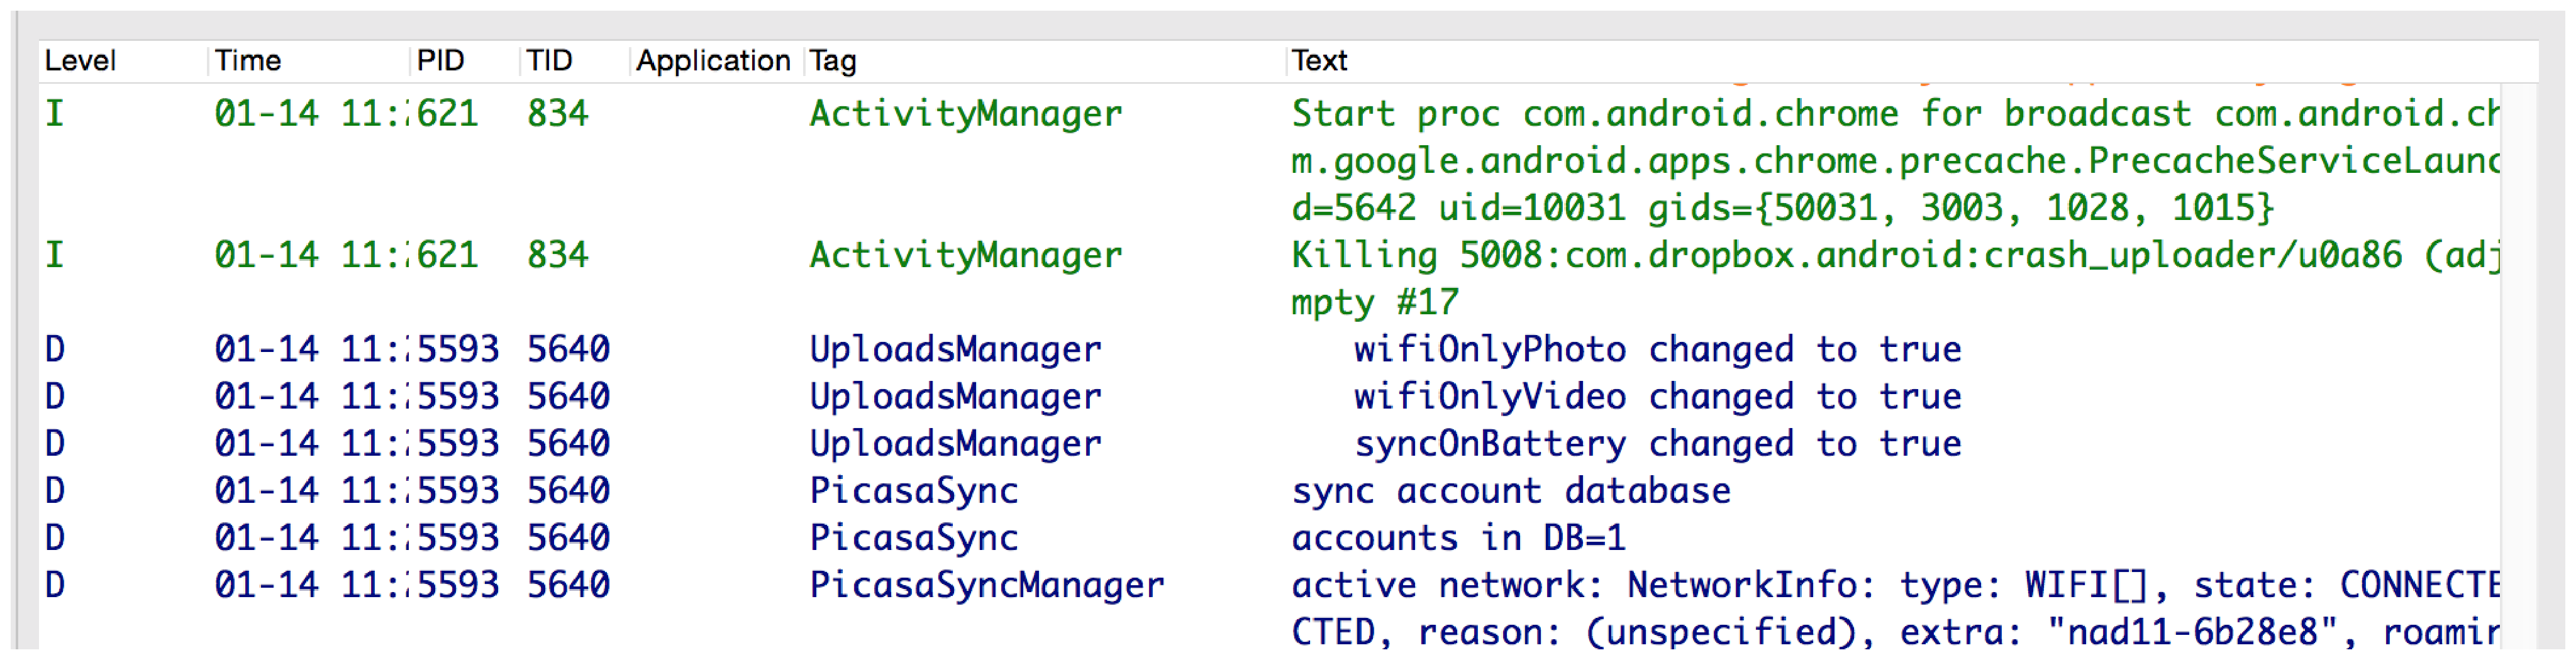
\includegraphics[scale=0.2]{androidlogexample.eps}
\end{center}
\caption{Android が出力するログの例}
\label{examplelog}
\end{figure}

\subsection{解析手順}
\label{analysismethod}
最初に,大まかな手順の流れを説明する.Step 1 で,APK ファイルから Java クラスファイルを取り出す. Step 2 では,その Java クラスファイルにログコードを挿入する.Step 3, 4  でそのログコードを挿入した APK ファイルを作成し,実機にインストールする.その後,マルウェアを起動して,ログを得る (Step 5, 6). 以下にそれぞれの Step の詳細な説明をする.

[Step1] まず最初の手順として,APK ファイルから Java クラスファイルを取り出す.\ref{sec:andrapp} で述べたように,APK ファイルを解凍することで,classes.dex を得ることができる.classes.dex からJava クラスファイルを取り出すために,dex2jar \cite{d2jar} が提供する sh プログラム (d2j-dex2jar.sh)を用いる.これにより, DEX コードファイルを JAR ファイルに変換することができる.よって,APK ファイルを解凍して出てきた classes.dex から dex2jar を用いて 1 つの JAR ファイルを得ることができる.この JAR ファイルを解凍することで Android アプリの Java クラスファイルを得る.

[Step 2] マルウェアの Java クラスファイルを得た後は,これにログを出力するコードを挿入する.つまりマルウェアの Java クラスファイルを書き換える.本研究では,Java クラスファイルを書き換えるために Javassist \cite{javassist} という Java ライブラリを用いる.Javassist は Java バイトコードの知識があまりなくても バイトコード変換のための API を提供する Java ライブラリである.Java で実装したプログラムでマルウェアの Java クラスファイルを書き換える.実装したプログラムについては,\ref{sec:instrument} 章で詳しく説明する.

[Step 3] Java クラスファイル を書き換えた後は,classes.dex を作成する.classes.dex を作成するためには,複数のクラスファイルを JAR ファイルにまとめる必要がある.dex2jar で得た JAR ファイルを解凍した際に,ディレクトリがいくつも出てくる場合がある.その場合は,ディレクトリ毎に JAR ファイルにまとめ,ディレクトリに属していないクラスファイルだけで,ひとつの JAR ファイルにまとめる. そして,以下に示すコマンドで JAR ファイルから classes.dex を作成する.dx とは,Android SDK が提供する dx コマンドのことである.このコマンドにより,JAR ファイルから DEX コードの変換を行う.

\begin{itembox}[l]{JAR ファイルから classes.dex を作る dx コマンド}
	dx --dex --output="classes.dex" "direcA.jar" "direcB.jar" 
\end{itembox}

[Step 4] 次に,新しく作成した classes.dex を APK ファイル内にあるオリジナルの classes.dex と入れ替え.端末にインストールできるように APK ファイルにサインを行う.先に述べたように,APK ファイルは ZIP 形式であるから, zip コマンドに -u オプションをつけることで,新しいファイルを古いものと入れ替えることができる.APK ファイルにサインするためには,dex2jar の中の d2j-apk-sign.sh を用いる.例えば,sampleApp.apk に対してこのプログラムを実行すると,sampleApp\_signed.apk のように別の新しい APK ファイルが生成される.そして,adb shell を使って,この APK ファイルを実機にインストールする.

[Step 5] マルウェアのインストール後,手動でそのマルウェアを起動し,DDMS に出力されるマルウェアのログをテキストファイルに保存する.Android OS が出力しているログは,ターミナルでも見ることができるが,細かい内部システムの状態などの情報が大量に出てくる.そのため,マルウェアが出しているログをそこから見つけることは困難である.DDMS では,指定したタグのみを出力することができる.マルウェアに挿入するコードには,タグを自分で指定しているため,DDMS にはマルウェアの実行ログのみを表示することができる.そして,表示されているログをテキストファイルとして保存する.

[Step 6] さらに,ログをより解析しやすくするために,このマルウェアのログのテキストファイルをクラス毎に分割する.なぜなら,そのままの状態では,複数のクラスのメソッドのログが混在していて,何が行われているか理解しにくいためだ.ログをパースするスクリプトを実装し,それを得られたテキストファイルに適用し,クラス毎に分割した.このスクリプトについては, \ref{sec:instrument} 章で詳しく説明する.

\subsection{ログコードの挿入箇所}
\label{placeinsert}
マルウェアの挙動を解析するためには,ログコードを適切な箇所へ挿入する必要がある.そこで本節では,マルウェアの Java クラスファイルへログコードを挿入する際に,どのような箇所へ挿入するか,どのような情報をログコードで出力させるかについて説明する.\ref{methodtop} では,メソッドの先頭へのコード挿入について,\ref{methodcalls} では,メソッド呼び出しの前後でのコード挿入について,なぜそこへ挿入するかという理由も含めて説明する.

\subsubsection{メソッドの先頭へのコードの挿入}
 \label{methodtop}
メソッドの先頭へログコードを挿入するのは,メソッドが実行された時に,そのログコードを確実に実行しそのログを出力させるためである.Javassist が提供する API では,メソッドの先頭か,最後にコードを挿入できる.メソッドの最後にコードを挿入してしまうと,メソッドが実行されたときに,そのコードが確実に実行されるかどうかは分からない.理由は主に 2 つ考えられる.1 つは,メソッドの途中で return 文が書かれている場合である.if 文の中で return 文が書かれていて,ある条件ではその if 文が実行されて,メソッドの最後まで到達せずに呼び出し元へ返ってしまい,メソッドの最後にあるログコードは実行されなくなってしまう.また,マルウェア作成者が解析者の混乱を誘うために,意図的にメソッドの途中で return 文を置いている可能性もある.もう一つの理由は,そのメソッドが途中で他のメソッドを呼び出してそのメソッドの最後まで到達しない場合だ.例えば メソッド A,B の最後にログコードを挿入し,メソッド A の中でメソッド B を呼びだすというケースを考える.そして,メソッド B の中でそのアプリが終了する関数が最後に呼ばれたとする.そうすると,メソッド A だけでなく,メソッド B のログコードも実行されなくなってしまう.なぜなら,メソッド B のログコードはアプリを終了させる関数の後に挿入されることから,このログコードは実行されないからだ.もし実行フローが最後まで到達して,ログコードが実行されたとしても,解析する際には時系列とは逆の順番でログが出力されるので紛らわしくなってしまうというデメリットもある.メソッドの先頭へログコードを挿入するイメージ図 \ref{insertbefore} を以下に示す.図 \ref{insertbefore} が示すように各メソッドのメソッド先頭,つまりそのメソッドが実行された場合,この挿入されたコードが一番最初に実行されるということになる.よって,メソッドの先頭にログコードを挿入すると,メソッド内の条件等にかかわらず,必ずそのログコードが実行されることになる.

\begin{figure}[t]
\begin{center}
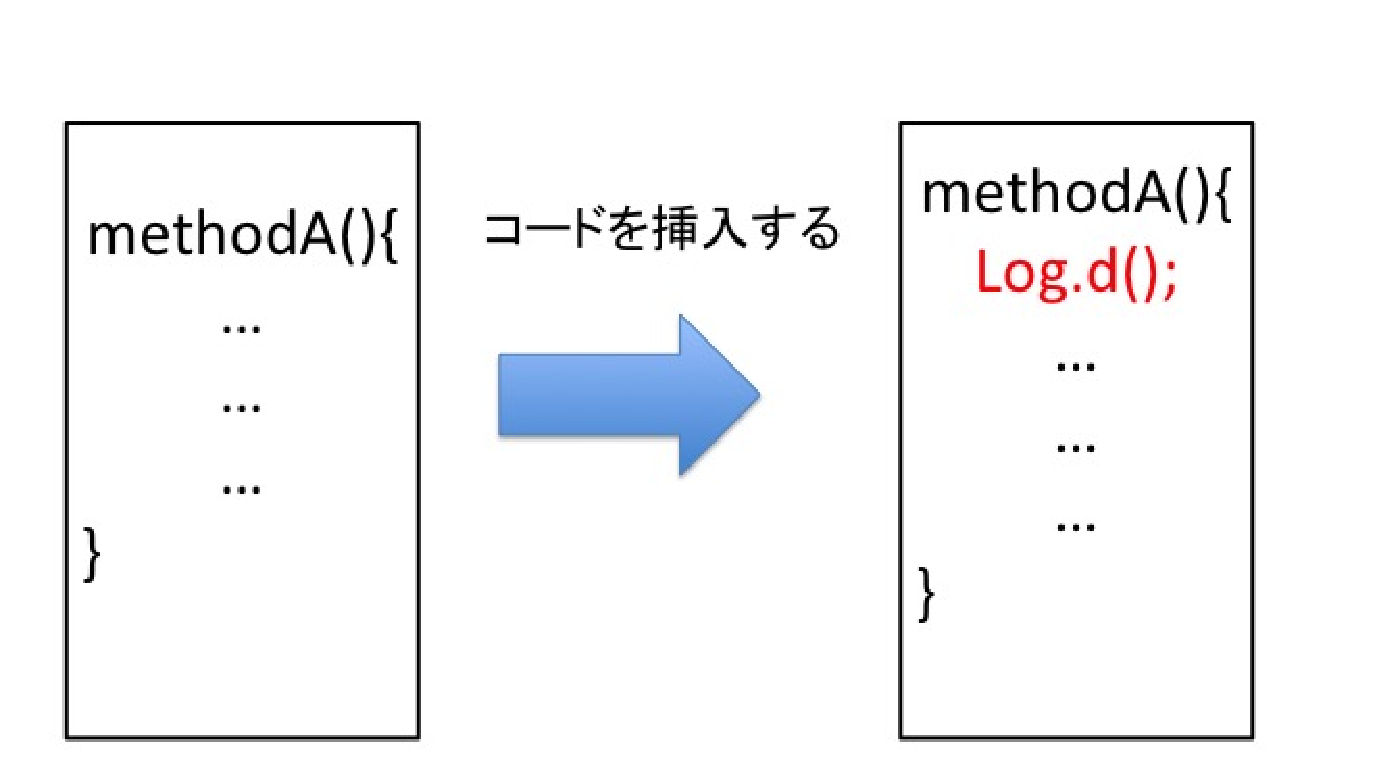
\includegraphics[scale=0.3]{image2.eps}
\end{center}
\caption{メソッドの先頭へコードを挿入するイメージ図}
\label{insertbefore}
\end{figure}

メソッドの先頭に挿入するログコードではクラス名,メソッド名,そのメソッドの引数の情報を出力させる.メソッドの引数の情報とは,引数の型名とその引数の値である.なぜ引数の型名だけでなく,中身を出力させるかというと,引数の中身がわかるとマルウェアの挙動がより見えやすくなるからである.例えば,メソッド名が "getCode",メソッドの引数の 1 つの型が String 型とわかっていたとする.しかし,これだけでは,String の中身がどんなものなのかよくわからない.なぜなら,String 型の変数はいろんな使われ方が考えられるからだ.型名だけで類推することはできても特定するのはとても困難である.この引数はサーバからのコマンドや,盗んだ端末についての情報の文字列かもしれない.そこで,引数の具体的な値が,URL のような文字列であることがわかると,この引数はコードを取ってくるアドレスということである確率がとても高いといえる.同様なことが int 型の場合も考えられる.もし int 型のメソッドの引数が携帯電話の番号(11 ケタで,090 や 080 で始まっている数字列)だった場合,そのマルウェアは感染した端末の電話番号を盗んでいたり,SMS をバックグラウンドで送信している可能性が出てくる.たとえメソッド名がマルウェア作成者により意図的に変えられていたとしても電話番号を引数にとっているということは端末の情報への不正なアクセスを明らかに示している.このようにメソッドの引数の値はマルウェアを解析するにあたって重要な要素であり,この情報によって解析がより行いやすくなる.

しかしこの手法を適用できないメソッドが 2 種類ある.
1 つは java.lang に属するクラスである.たとえば,String クラスのメソッドである,toString() の先頭にはログコードを挿入することはできない.Javassist の API では,JVM にすでにロードされているクラスのクラスファイルは書き換えることができないという制限がある.そのため,Java のプログラムが実行時(この場合,クラスファイルを書き換えようとしている時)には,JVM には java.lang.String クラスがロードされているため,Javassist は String  クラスのクラスファイルを書き換えることはできない.この手法を適用できないもう一つのメソッドの種類は Android API である.Android API は Android システムの内部に組み込まれているため,Java クラスファイルとしては存在していない.Javassist は Android の内部に組み込まれているものを操作できないため,Javassist では,これらのメソッドの先頭にコードを挿入することはできない.マルウェアをより詳細に解析していくためには,メソッドの先頭へログコードの挿入は不十分である.この問題を解決するために, \ref{methodcalls} の手法を利用する.

\subsubsection{メソッド呼び出しの前後でのコードの挿入}
\label{methodcalls}
マルウェアをより深く解析していくために,メソッド呼び出しの前後にログコードを挿入する.図 \ref{insertbetw} はメソッドの前後にコードを挿入するイメージ図である.この図が示すように,呼び出されるそれぞれのメソッドの前後にログコードを挿入する.
この図では,methodA の中で,methodB, methodC が呼び出されている.methodA が実行されたとすると,methodB, methodC の実行の前後にそれぞれのメソッドについてのログが出力されることになる.つまり,あるメソッド内でどのようなメソッドが呼び出されているかがわかるようになる.

メソッドの前後にログコードを挿入する場合は \ref{methodtop} の手法とは異なる Javassist の API を用いるため,\ref{methodtop} の手法では適用できない2 種類のメソッドについてのログを出力することができる.つまり,あるメソッドの中で java.lang のクラスのメソッドや,Android API が実行されたということがわかるようになる.図 \ref{insertbetw} の methodB または methodC が java.lang.String  クラスの toString() であってもこの手法を適用することができる.メソッド呼び出しの前後にログコードを挿入することで,より多くのメソッドについてのログが出せるようになり,あるメソッド内でどんなメソッドが実行されたかが明らかになる.

\begin{figure}[t]
\begin{center}
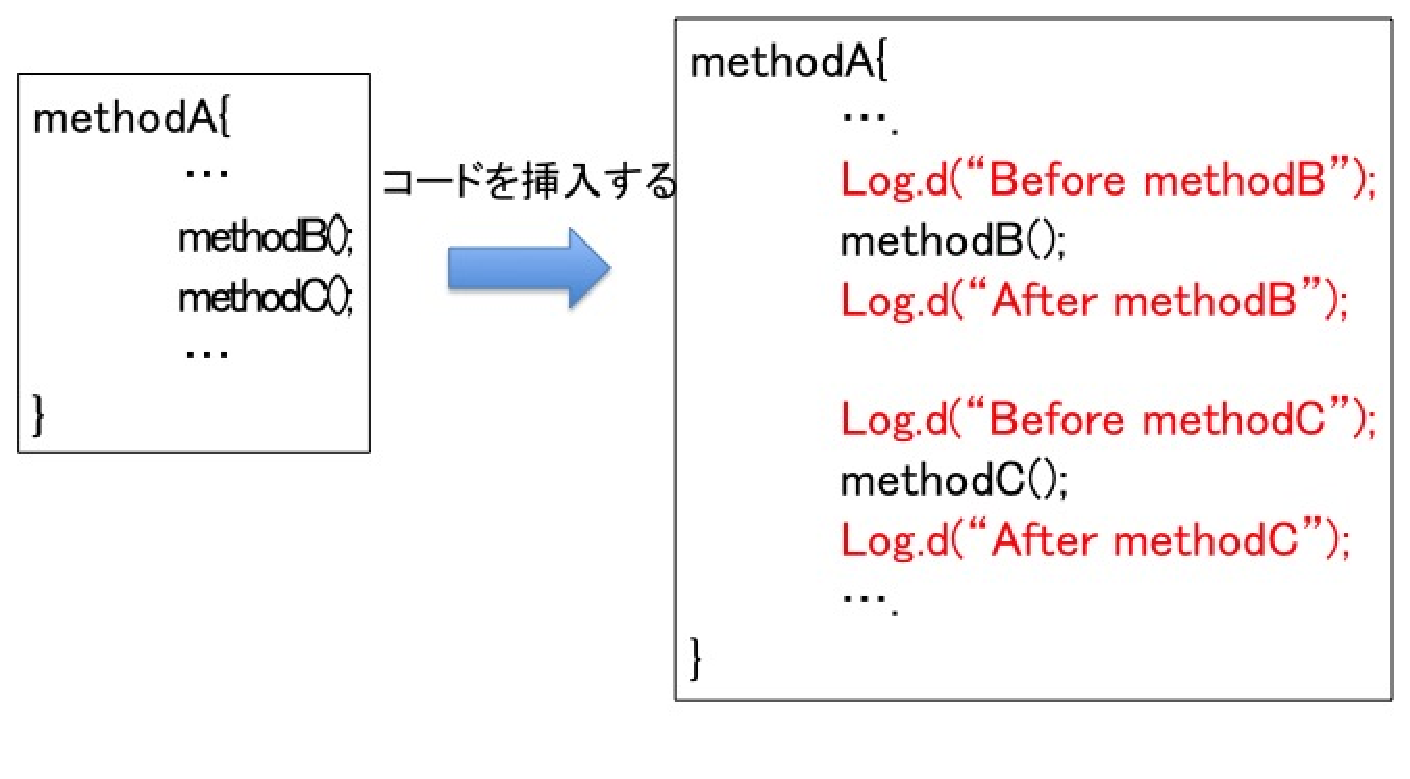
\includegraphics[scale=0.35]{image4.eps}
\end{center}
\caption{メソッドの前後にコードを挿入するイメージ図}
\label{insertbetw}
\end{figure}

\begin{figure}[t]
\begin{center}
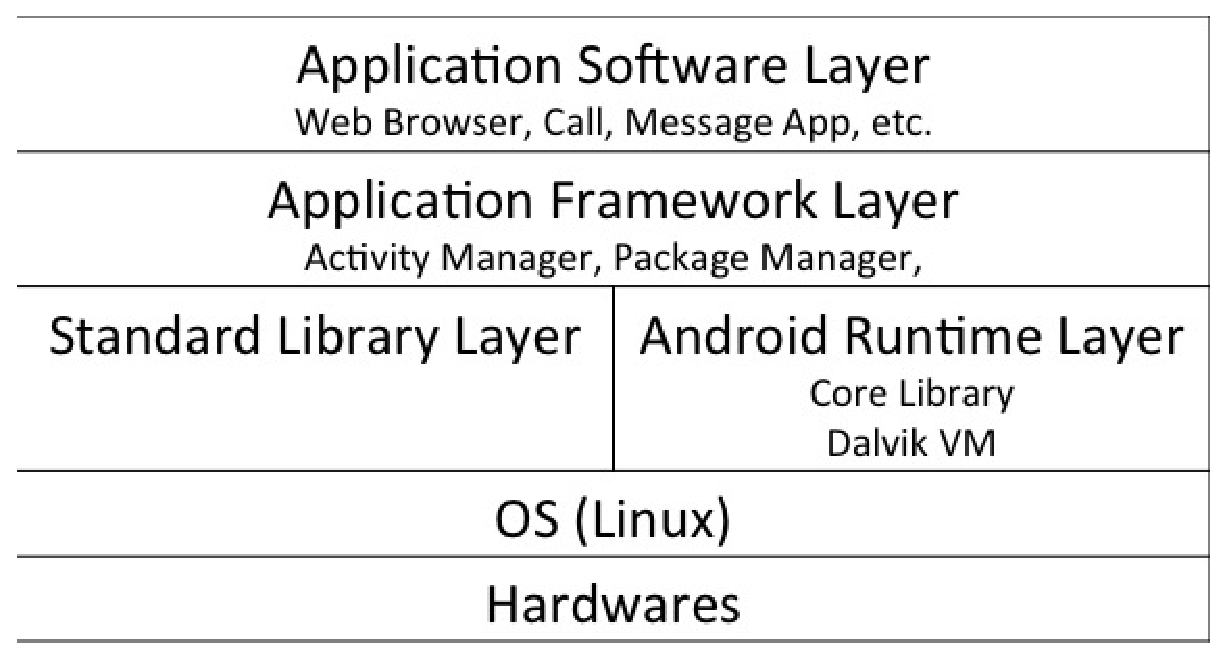
\includegraphics[scale=0.5]{structure2.eps}
\end{center}
\caption{Android の内部構成}
\label{structure}
\end{figure}

呼び出されるメソッド呼び出しについてのログには,それ自身はもちろんのこと,呼び出し元のメソッドの情報も出力させる.呼び出し元のメソッドの情報はマルウェアの解析に必要である.なぜなら,マルウェアの解析を行うにあたり,どのメソッドがどこから呼び出されたかを知る必要があるからだ.どこから呼び出されたかがわからないと,ただそのメソッドが実行されたということしかログからは知り得ない.例えば,クラス A のメソッド mA とクラス C のメソッド mC の 2 つのメソッドからクラス B の mB が実行される場合を考える.もし,呼び出し元の情報がないと,クラス B の mB の実行ログを得ても,クラス A のメソッド mA からなのか,クラス C のメソッド mC から呼び出されているかがわからない.

また,\ref{methodtop} の方法では,プログラムの実装の都合や Javassist のAPI の都合上,呼び出し元をログとして出力させることはできない.\ref{sec:instrument} 章で説明するように,メソッドの先頭に挿入するプログラムのアルゴリズムでは,呼び出し元の情報を得る機能を追加することはできないためだ.この場合については,メソッドへのコードを挿入せずに,メソッド呼び出しの置き換えを行っている.この置換えによって,メソッドのオブジェクト(javassist.expr.MethodCall クラスのオブジェクト ) を得られる.MethodCall クラスのオブジェクトの情報から呼び出しているメソッド名,そのメソッドのクラス名を取得することができる.


\clearpage

\section{実装}
\label{sec:instrument}
本章では,本提案をマルウェアに適用するために実装したプログラムについて説明する.
\ref{programforclass}では,Java ウラスファイルを書き換えるためのプログラムについて,\ref{splitscript}では,DDMS で得られたログを処理するためのプログラムについて擬似コードやソースコードを交えながらそのアルゴリズムや実行の流れを解説する.

\subsection{Java クラスファイルを書き換えるためのプログラム}
\label{programforclass}
\ref{methodtop}, \ref{methodcalls} で提案した手法を実現するためには,Javaクラスファイルを操作したり,中身を見る必要がある.
Java クラスファイルは c 言語のプログラムがコンパイルされて生成される実行ファイルのようにバイナリーコードではないため,人間が読み取ることはできる.
しかし,Java ファイル (.java のファイル) の中身とクラスファイルを対応させるためには,Java バイトコードの知識が必要であり,時間がかかってしまう.
クラスファイルを編集するためには Java バイトコードについてさらに深く知る必要がある.
また,クラスファイルを自分で直接編集しても文法エラー等により JVM もしくは Dalvik VM で正しく実行できない可能性もある.
特に Java バイトコードから DEX コードへの変換や DEX コードについての情報はまだ少なく,そのデバッグ作業は非常に難しいといえる.
このような理由から Javassist\cite{javassist} を用いたプログラム が必要である.

Javassist の API を使うことで,Java バイトコードについての知識や,Java バイトコードとDEX コードの変換を気にすることなく,クラスファイルを扱うことができる.
つまり,Java クラスファイルをメソッドひとつで書き換えたり,クラスファイルの中身について知ることができる.
クラスファイルの情報とは,メソッド名やクラス名,メソッドの引数の型名のことである.
このように,Java で実装したプログラムを使って,クラスファイルを書き換えることができる.

また,jad\cite{jad}というツールを使うことで,Java クラスファイルを Java ファイルに逆コンパイルすることもできる.
jad はクラスファイル (.class) から jad ファイル (.jad)を生成する.
jad ファイルの中身は Java ファイルと同じだが,拡張子のみが異なる.
今回の実装では,Java クラスファイルが書き換えられたかどうかを確認するためにこのツールを用いた.

\ref{methodtop}と,\ref{methodcalls} で提案する手法では,それぞれ Java クラスファイルを操作する方法が異なるため,別々に説明する.

\subsubsection{メソッドへのコードの挿入}
\label{insertcodes}
マルウェアに限らず,Android のアプリのソースコードは多くのクラスから構成されている.
例えば,ある辞書アプリのクラスファイルの数は 120 を超える.
全てのクラスにコードを挿入してしまうと,膨大なログがでてきてしまうため,コードを挿入するクラスを選定する必要がある.
クラスを選定するためには,それぞれのクラスファイルについて中身を知らなければならない.
このような多数のクラスファイルをひとつひとつ逆コンパイルして中身を確認してからクラスファイルを書き換えていては非常に効率が悪い.
また,実行時におけるメソッドの引数の値を表示するためには Javassist の機能を用いることで実現できる.
そこで,複数のクラスファイルのメソッドへコードを挿入するためのプログラムを実装した.

まず,このプログラムの全体の流れを説明する.
コードを挿入する前の準備として,不正な動きをすると思われるメソッドを持つクラスを探し出す,
"download", "install", "command" などマルウェアの不正な動きを表すキーワードでメソッドを検索し,このキーワードを含んだメソッドをもつクラス名を取得する.
ここで取得したクラスがコードを挿入するクラスとなる.
最初に,コードを挿入するクラス名をコマンドラインから入力する.
次に,入力したクラス名に一致するクラスをそのアプリのディレクトリー内のクラスファイルから検索する.
最後に,検索により見つかったクラスのそれぞれのメソッドへログコードを挿入する.
%図はこのプログラムの擬似コードである.

最後のステップで挿入するコードはそのメソッド名,クラス名,そしてそのメソッドの引数の型名とその値を出力させるコードである.
メソッドの引数の実行時の値はクラスファイルを書き換えるときには分かり得ないため,特別な処理が必要である.
そこで,メソッドの引数の値を表示するために Javassist の特殊変数を用いる.
%insertBefore(String str) というメソッドでメソッドの先頭にコードを挿入する..
図\ref{insert before}は メソッドの先頭にコードを挿入する Javassist のメソッドの insertBefore の使用例である.
この図中の m は挿入するメソッドを表すオブジェクト (javassist.CtMethod) で,\$args[0], \$args[1] は, Javassist の特殊変数で,メソッドの引数を表す.
insertBefore の引数の文字列は挿入するコードの文字列である.
例えば,オブジェクト m が図\ref{vector}のクラス MyVector のメソッド add を表しているとする.
insertBefore の実行後は図 のようになって,\$args[0], \$args[1]がそれぞれ dx, dy に置き換わる.
つまり,add メソッドの引数を表示することができる.
メソッドによっては引数の数が異なるので,それぞれのメソッドの引数の個数を取得して,その数に合わせて挿入するコードを生成した.

\begin{figure}[t]
\begin{center}
\graphicspath{{./epsfiles/}}
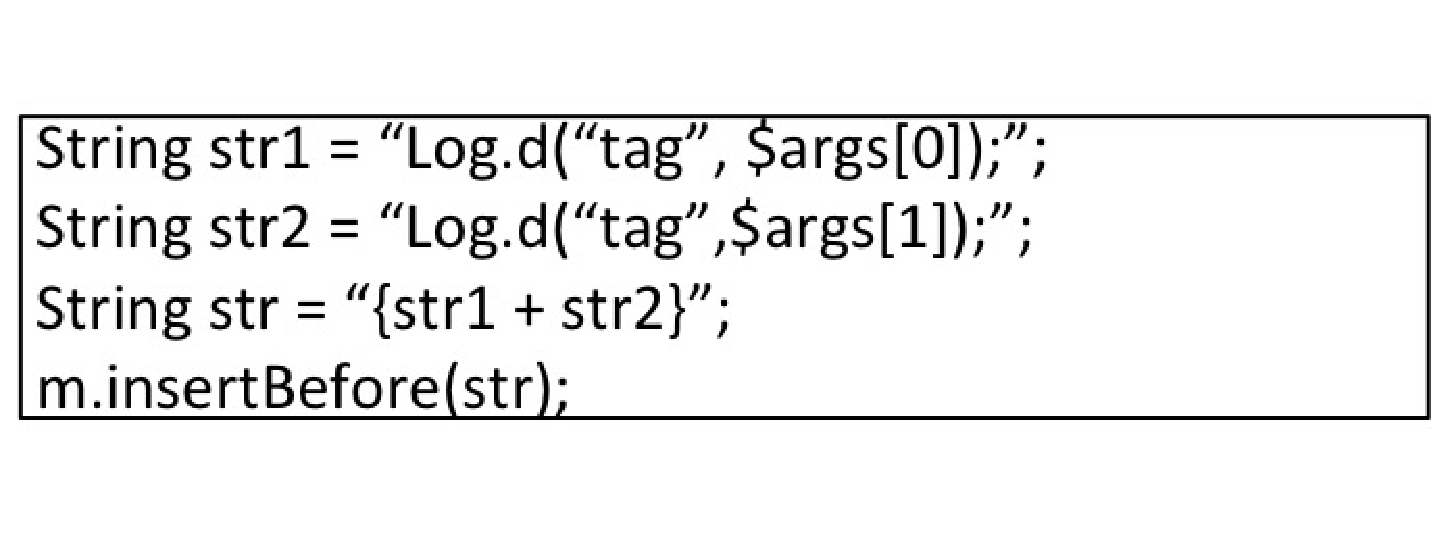
\includegraphics[scale=0.3]{insertbefore2.eps}
\end{center}
\caption{CtMethod.insertbefore の使用例}
\label{insertbefore}
\end{figure}


\begin{figure}[t]
\begin{center}
\graphicspath{{./epsfiles/}}
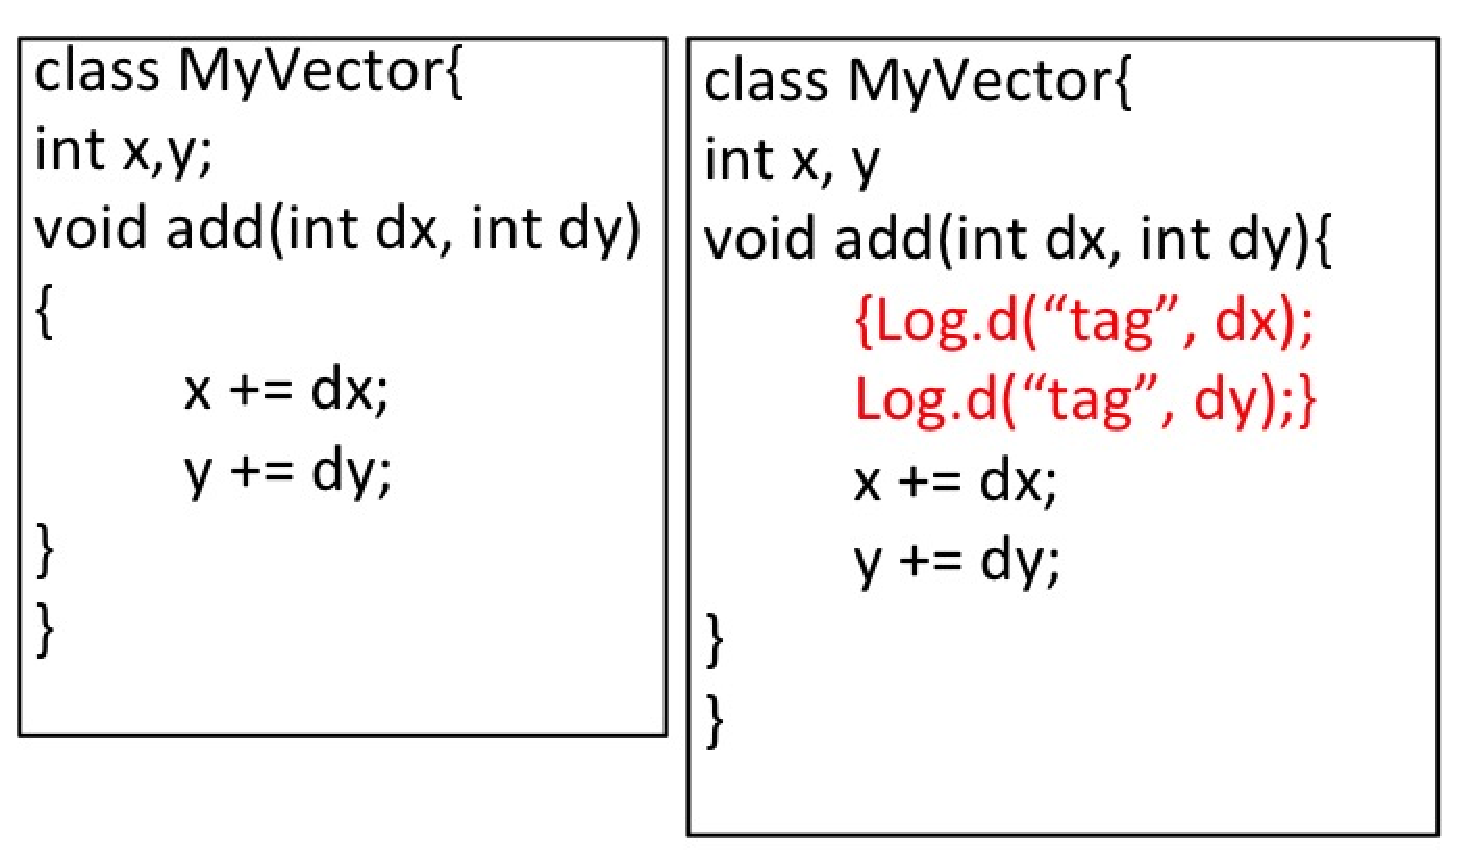
\includegraphics[scale=0.3]{vector.eps}
\end{center}
\caption{insertBefore 実行前後の MyVector クラス}
\label{vector}
\end{figure}

\subsubsection{メソッド呼び出しの置き換え}
\label{replacement}
\ref{methodcalls} の提案を実現するために,メソッドの置き換えを行う.
\ref{methodcalls} では,メソッドの前後にコードを挿入すると述べたが,この場合には,\ref{insertcodes} で説明した insertBefore を用いることはできない.
なぜなら,この場合はメソッドの先頭ではなく,それぞれのメソッド呼び出しの前後にコードを挿入するためである.
そのため, コードの置き換えを行う別のメソッドを用いる.

 Javassist のメソッドの replace によりメソッド呼び出しの置き換えを行う.
図\ref{replace}はこのメソッドの使用例である.
図中の m はメソッド呼び出しを表すオブジェクト (javassist.expr.MethodCall) である.
ある methodA の中の method1 が m だったとすると,図\ref{methoda}のようになる
"\$\_= \$proceed(\$\$);" は置換される元のコードを実行する文である.
\$, \$proceed, \$\$ も \$args と同様,Javassist の特殊変数である.
\$\_ は置換される元のコードの計算結果,\$proceed は置換される前の呼び出されるメソッド名 (図  では method1 となる), \$\$ は元のメソッド呼び出し式の引数列を表す.

メソッド呼び出しの前後に入るログコードには,次に示す情報を出力させるコードである.
1. 呼び出されるメソッドの名前,2. そのメソッドのクラス,3. 返り値の型,4. 引数の型,5. 呼び出しているメソッド名,を含んだ文字列を作る.
この文字列を図\ref{replace}の str1 の "before", str3 の "after" にあたる場所へ代入する.
これらの情報は Javassist の API を用いることで取得できる.

メソッド呼び出しを置き換えるプログラムの全体の流れは\ref{insertcodes}と同様である.
前処理として,コードを挿入するクラスを決定する.
そして,入力されたクラスを検索し,見つかったクラスのそれぞれのメソッドに対して先に述べた replace による置き換えを行う.

\begin{figure}[t]
\begin{center}
\graphicspath{{./epsfiles/}}
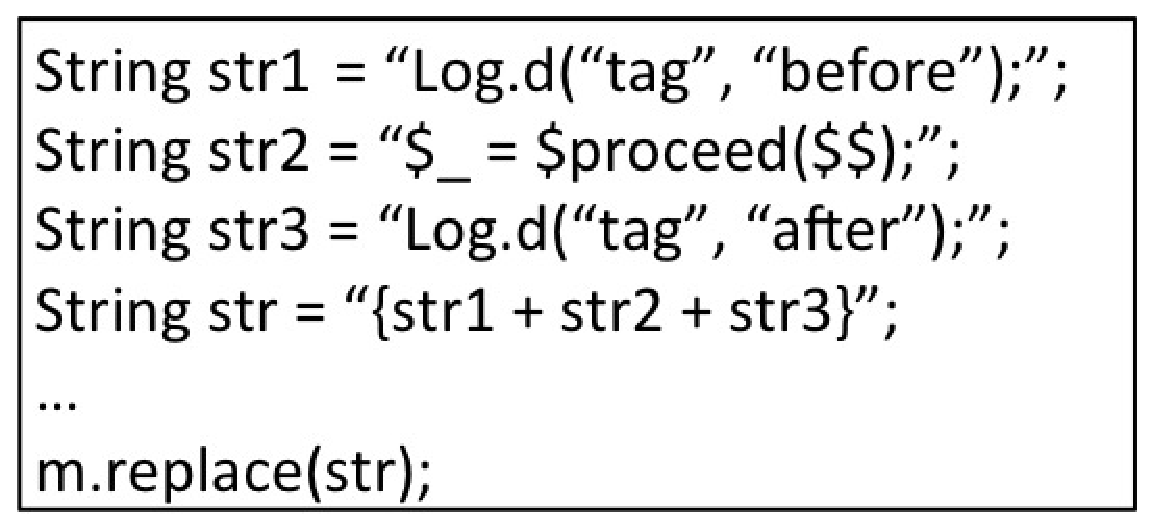
\includegraphics[scale=0.3]{replace.eps}
\end{center}
\caption{MethodCall.replace の使用例}
\label{replace}
\end{figure}

\begin{figure}[t]
\begin{center}
\graphicspath{{./epsfiles/}}
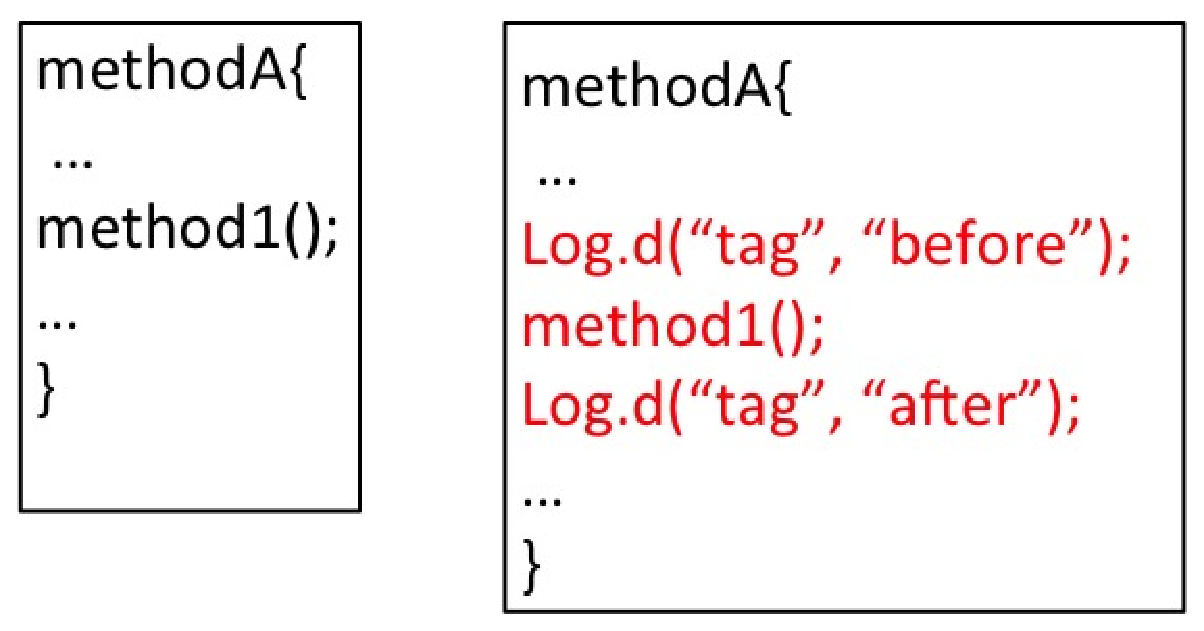
\includegraphics[scale=0.3]{methoda.eps}
\end{center}
\caption{replace 実行前後の metthodA メソッド}
\label{methoda}
\end{figure}

\subsubsection{private メソッドを書き換える方法}
\label{private}
\ref{insertcodes} で 
private メソッドにコードを挿入する方法は public メソッドとは異なる.
Javassist の中で,クラスを表すオブジェクト javassist.CtClass がある.
CtClass のメソッド getMethods はそのクラスが持つメソッド (CtMethod) の配列を返す.
しかし,private メソッドは getMethods の返り値の配列には入らない仕様となっている.
\ref{insertcodes}, \ref{replacement} では,getMethods で返されたメソッドのみに対してコードを挿入した.
より詳細なログを得るためには private メソッドを書き換える必要がある.

この解決策は,\ref{replacement}のプログラムで得たログからprivate メソッド名とそのクラス名を取得することだ.
\ref{replacement}のプログラムでは,private メソッドの前後にもログを挿入することが可能である.
メソッド名とそのクラス名がわかっていれば,そのメソッドのアクセス修飾子を変えることができる.
この場合,CtMethod オブジェクトを自分で宣言することができるため,getMethods を用いることなく,CtMethod オブジェクトを得ることができる. 
よって,CtMethod クラスのメソッドである,setModifier を用いて private から public に変えることができる.

なお,もともと private であったメソッドを public にした場合,private に戻す必要がある.
public にしたままで Android の実機で実行したところ,インストールはできたが,アプリを実行できなかった.
この時に Android OS が出したログには,実行が失敗した原因は private なメソッドが public になっているためと説明されていた.
そのため,private から public にしたメソッドを元に戻した(private に戻して) ところ,正常に動作した.

\subsection{得られたログを処理するためのプログラム}
\label{splitscript}
目的

比較

\begin{itembox}[c]{DDMS より得られたログの一部}
\footnotesize{
%\begin{verbatimtab}[4]
12-17 15:07:40.063: D/(12568): CLASS: com.mj.iMatch.IMatch METHOD: onCreate args[0]:android.os.Bundle = null\\
12-17 15:07:40.063: D/(12568): ID: 321 Before onCreate Called From onCreate In com.mj.iMatch.IMatch\\
12-17 15:07:40.063: D/(12568): ID: 321 After onCreate Backed To onCreate In com.mj.iMatch.IMatch\\
...\\
12-17 15:07:40.063: D/(12568): ID: 55 After getDefaultDisplay Backed To  onCreate In com.mj.iMatch.IMatch\\
12-17 15:07:40.063: D/(12568): CLASS: com.mj.iMatch.CommonUtils METHOD: setDisplay args[0]:android.view.Display = Display id 0: DisplayInfo{"Built-in Screen", app 1080 x 1776, real 1080 x 1920, largest app 1794 x 1701, smallest app 1080 x 1005, 60.0 fps, rotation0, density 480 (442.451 x 443.345) dpi, layerStack 0, type BUILT\_IN, FLAG\_SECURE, FLAG\_SUPPORTS\_PROTECTED\_BUFFERS}, DisplayMetrics{density=1.0, width=320, height=526, scaledDensity=1.0, xdpi=147.48367, ydpi=147.78168}, isValid=true\\
12-17 15:07:40.063: D/(12568): ID: 688 Before getWidth Called From setDisplay In com.mj.iMatch.CommonUtils\\
12-17 15:07:40.063: D/(12568): ID: 688 After getWidth Backed To  setDisplay In com.mj.iMatch.CommonUtils\\
12-17 15:07:40.063: D/(12568): ID: 741 Before getHeight Called From setDisplay In com.mj.iMatch.CommonUtils\\
12-17 15:07:40.063: D/(12568): ID: 741 After getHeight Backed To  setDisplay In com.mj.iMatch.CommonUtils\\
12-17 15:07:40.083: D/(12568): ID: 184 Before setContentView Called From onCreate In com.mj.iMatch.IMatch\\
12-17 15:07:40.133: D/(12568): CLASS: com.admob.android.ads.AdManager METHOD: isEmulator args[]: No Parameter\\
12-17 15:07:40.133: D/(12568): ID: 647 Before equals Called From isEmulator In com.admob.android.ads.AdManager\\
12-17 15:07:40.133: D/(12568): ID: 647 After equals Backed To  isEmulator In com.admob.android.ads.AdManager\\
....\\
12-17 15:07:40.183: D/(12568): ID: 455 Before loadPreferences Called From onResume In com.mj.iMatch.IMatch\\
12-17 15:07:40.183: D/(12568): CLASS: com.mj.iMatch.IMatch METHOD: loadPreferences args[]: No Parameter\\
12-17 15:07:40.183: D/(12568): ID: 12 Before getSharedPreferences Called From loadPreferences In com.mj.iMatch.IMatch\\
12-17 15:07:40.183: D/(12568): ID: 12 After getSharedPreferences Backed To  loadPreferences In com.mj.iMatch.IMatch\\
12-17 15:07:40.183: D/(12568): ID: 667 Before getInt Called From loadPreferences In com.mj.iMatch.IMatch\\
12-17 15:07:40.183: D/(12568): ID: 667 After getInt Backed To  loadPreferences In com.mj.iMatch.IMatch\\
12-17 15:07:40.183: D/(12568): ID: 455 After loadPreferences Backed To  onResume In com.mj.iMatch.IMatch\\
%\end{verbatimtab}
}
\end{itembox}


\begin{itembox}[c]{クラスごとに分けたログの一部}
\footnotesize{
\begin{verbatimtab}[4]
0 CLASS com.mj.iMatch.IMatch METHOD onCreate args[0]android.os.Bundle = null
1	 ID 321 Before onCreate Called From onCreate In com.mj.iMatch.IMatch
2	 ID 321 After onCreate Backed To  onCreate In com.mj.iMatch.IMatch
...
76	 ID 455 Before loadPreferences Called From onResume In com.mj.iMatch.IMatch
77	 CLASS com.mj.iMatch.IMatch METHOD loadPreferences args[] No Parameter
78		 ID 12 Before getSharedPreferences Called From loadPreferences 
In com.mj.iMatch.IMatch
79		 ID 12 After getSharedPreferences Backed To  loadPreferences 
In com.mj.iMatch.IMatch
80		 ID 667 Before getInt Called From loadPreferences In com.mj.iMatch.IMatch
81		 ID 667 After getInt Backed To  loadPreferences In com.mj.iMatch.IMatch
82	 ID 455 After loadPreferences Backed To  onResume In com.mj.iMatch.IMatch

\end{verbatimtab}
}
\end{itembox}

\clearpage

\section{実験}
\label{sec:exp}
提案手法をマルウェアに適用して実験を行った.本章では,この実験の目的,方法,結果について解説する.
\subsection{実験の目的}
本研究の提案手法により得たマルウェアの実行ログから,マルウェアの挙動を明らかにできていることを示す.

\subsection{実験方法}
今回,11 個の検体を用いた実験と,SMS を送るマルウェア (1 つのマルウェア)を用いた実験の 2 種類の実験を行った.実験の説明の前に \ref{expmalware} で,実験に用いたマルウェアがどのような挙動を示すかを示す.それぞれの実験については, \ref{exp1} , \ref{exp2} で詳しく説明する.

\subsubsection{実験に用いたマルウェア}
\label{expmalware}
今回の実験に用いたマルウェアの挙動を以下に示す \cite{golddream} \cite{basebridge} \cite{droiddreamlight} \cite{crazyapp} \cite{icalendar} \cite{snake} \cite{trojan} .

\begin{enumerate}
\item GoldDream
	\begin{itemize}
	\item	receiver を使うことで,SMS,電話等のシステムイベントをバックグラウンドで監視し,送信元のアドレス,電話,SMS のタイムスタンプ,電話番号をファイルに保存した後,外部のサーバへそのファイルを送信する.
	\item 外部のサーバから 4 種類のコマンドを受け取り,それを実行する.
	\begin{enumerate}
		\item SMS をバックグラウンドで送信する
		\item 電話を発信する
		\item アプリをインストールまたはアンインストールする
		\item ファイルを外部のサーバへアップロードする
	\end{enumerate}
	\end{itemize}

\item basebridge
	\begin{itemize}
	\item アプリのアップグレードを促すダイアログを出し.そこでアップグレードを選択すると,basebridge は com.android.battery を感染した端末にインストールする.
	\item 外部のサーバとの通信を行い,番号などが載った configuration list  をダウンロードし,この情報を基に,SMS を送信する.
	\item SMS をバックグラウンドで送信したことをユーザに気付かれないようにするために,モバイルキャリアからの課金確認の SMS をブロックする.
	\end{itemize}

\item com.tencent.qqgame
	\begin{itemize}
	\item 挙動は GoldDream と同じ
	\end{itemize}

\item Beauty Breast
	\begin{itemize}
	\item 感染した端末に電話がかかってくると,その端末の端末番号,機種名,SDK バージョン等の端末の情報を外部サーバへ送る.
	\item 新しいパッケージのインストールと,それを促すプロンプトを表示する.
	\item マルウェア自身では,上の挙動をすることはなく,ユーザの何らかの操作無しでは実行されない.
	\end{itemize}

\item Beauty Leg
	\begin{itemize}
	\item Beauty Breast と挙動は同じ
	\end{itemize}

\item Beauty Girl
	\begin{itemize}
	\item Beauty Breast と挙動は同じ
	\end{itemize}

\item crazy app
	\begin{itemize}
	\item 感染した端末の IMEI (端末を識別する番号) を外部サーバへ送信する.
	\item  ブラウザのブックマーク情報とブラウザの閲覧履歴をアップロードする.
	\end{itemize}
\item iCalendar
	\begin{itemize}
	\item 有料サービスに登録させるためにある番号へ SMS をバックグラウンドで送信する.
	\item SMS  を送信できたかどうかをタグとして内部で記録している.
	\item ユーザに気づかれるのを防ぐために一度しか行われない.
	\end{itemize}
	
\item iMatch
	\begin{itemize}
	\item 挙動は iCalendar と同じだが,SMS は起動する度に何度も送信される.
	\end{itemize}
	
\item Snake App
	\begin{itemize}
	\item バックグラウンドで外部サーバに端末の GPS 情報を送信する.
	\item 表向きはゲームアプリとして振舞っている.
	\end{itemize}
	

\item com.tencent.qq
	\begin{itemize}
	\item 感染した端末の IMEI 番号,電話番号,登録者 ID,SIM カードのシリアル番号を盗み,外部のサーバへ送信する.
	\item 過去に SMS を送った電話番号を収集する.
	\item 外部のサーバからコマンドを受け取り,以下の動作を行う
	\item SMS コンテンツや URL をサーバから受け取った電話番号へ送信する.
	\item ある URL から APK ファイルをダウンロードし,それをインストールする.
	\item ブラウザにブックマークを追加する.
	\item ある URL へ誘導するポップアップを表示する.
	\item ログファイルに記載されている電話番号からの SMS をブロックする.
	\end{itemize}
\end{enumerate}

\subsubsection{11 個の検体を用いた実験}
\label{exp1}


\subsubsection{SMS  を送るマルウェアの実験}
\label{exp2}

\subsection{実験結果}

\clearpage

\section{おわりに}
\label{sec:concl}
おわりに
\subsection{まとめ}

\subsection{今後の課題}
SIM カードを挿入してみる
Android API のログを得る.
自分でビルドする.
\clearpage

\section*{謝辞}
\addcontentsline{toc}{section}{謝辞}
本研究を行うにあたり,真摯に向き合ってくださり,たくさんのご指導を頂いた河野健二准教授に心から深く感謝申し上げます.また,河野研究室の皆様にも,日頃から多大な支援をいただいたことにつきまして,この場をお借りして感謝します.
\clearpage

\addcontentsline{toc}{section}{\numberline{}参考文献}
\bibliographystyle{junsrt}
\bibliography{reference}
%\clearpage

\end{document}

